\documentclass{article}
\usepackage[utf8]{inputenc}
\usepackage[T1]{fontenc}
\usepackage[spanish,es-tabla,es-noshorthands]{babel}

\usepackage{amsmath}
\usepackage{amssymb}
\usepackage{icomma} % coma decimal sin espacio en modo matemático

\usepackage{graphicx}
\usepackage{float}
\usepackage{caption}
\usepackage{subcaption}

\usepackage{booktabs}
\usepackage{array}
\usepackage{longtable}
\usepackage{tabularx}

\usepackage[margin=2.5cm]{geometry}
\usepackage{xcolor}
\usepackage{tikz}
\usetikzlibrary{arrows.meta,positioning,calc,babel}

\usepackage{algorithm}
\usepackage{algpseudocode}
\floatname{algorithm}{Algoritmo}
\renewcommand{\algorithmicrequire}{\textbf{Entrada:}}
\renewcommand{\algorithmicensure}{\textbf{Salida:}}

\usepackage[hidelinks]{hyperref}

\definecolor{flujo}{HTML}{2A78D6}
\definecolor{greedy}{HTML}{EB6834}
\definecolor{manual}{HTML}{1BAF7A}
\definecolor{gris}{HTML}{8A8983}

% cifras generadas por generar_figuras.py (ninguna se transcribe a mano)
\newcommand{\redNodos}{723}
\newcommand{\redAristas}{1677}
\newcommand{\redMs}{115}
\newcommand{\redPasadaUno}{127}
\newcommand{\redPasadaDos}{0}
\newcommand{\pesoA}{0,16}
\newcommand{\pesoB}{0,12}
\newcommand{\pesoC}{0,12}
\newcommand{\pesoD}{0,6}
\newcommand{\propA}{0,4}
\newcommand{\propB}{0,3}
\newcommand{\propC}{0,3}
\newcommand{\fAlumnos}{77}
\newcommand{\hAlumnos}{75}
\newcommand{\gAlumnos}{77}
\newcommand{\fTres}{16}
\newcommand{\hTres}{14}
\newcommand{\gTres}{14}
\newcommand{\fCob}{100,0}
\newcommand{\gCob}{99,2}
\newcommand{\gCubiertos}{126}
\newcommand{\fNoEleg}{1}
\newcommand{\hNoEleg}{6}
\newcommand{\gNoEleg}{4}
\newcommand{\hChoques}{3}
\newcommand{\fPrimProf}{63,0}
\newcommand{\hPrimProf}{71,7}
\newcommand{\gPrimProf}{89,7}
\newcommand{\fTresProf}{96,9}
\newcommand{\fPromAlum}{3,67}
\newcommand{\hPromAlum}{5,18}
\newcommand{\fNotas}{41,7}
\newcommand{\hNotas}{26,0}
\newcommand{\fCosto}{9,83}
\newcommand{\hCosto}{16,73}
\newcommand{\gCosto}{13,42}

\newcommand{\ofCupos}{218}
\newcommand{\ofFlujo}{164}
\newcommand{\ofFlujoPct}{75,2}
\newcommand{\ofGreedy}{162}
\newcommand{\ofHist}{127}
\newcommand{\ofSinCubrir}{54}
\newcommand{\ofSinPost}{53}
\newcommand{\ofSinPostLab}{35}
\newcommand{\ofNoRank}{7}
\newcommand{\ofNoEleg}{3}

\newcommand{\casoSigla}{CIT2011}

\newcommand{\elegPromMin}{5,0}
\newcommand{\elegNotaMin}{5,0}
\newcommand{\elegPostNo}{251}
\newcommand{\elegPostTotal}{1.245}
\newcommand{\elegAlumNoProm}{25}
\newcommand{\elegHistNo}{6}
\newcommand{\sinRankSecciones}{5}
\newcommand{\sinRankPost}{69}

\newcommand{\libreA}{0,3}
\newcommand{\libreB}{0,3}
\newcommand{\libreC}{0,4}
\newcommand{\jerA}{0,4}
\newcommand{\jerB}{0,3}
\newcommand{\jerC}{0,3}
\newcommand{\pesosN}{66}
\newcommand{\pesosSemillas}{10}
\newcommand{\jerPrimProf}{63,0}
\newcommand{\librePrimProf}{56,3}
\newcommand{\jerTresProf}{96,7}
\newcommand{\libreTresProf}{92,8}

\newcommand{\neExcluirCub}{126}
\newcommand{\neDosCub}{127}
\newcommand{\neDosNo}{1}
\newcommand{\nePenChicoNo}{5}
\newcommand{\nePenGrandeNo}{1}
\newcommand{\nePenMedioNo}{2}
\newcommand{\neSinCritNo}{7}
\newcommand{\neDCritico}{0,6}

\newcommand{\capDosAlumnos}{82}
\newcommand{\capDosCub}{127}
\newcommand{\capDosPrim}{59,1}
\newcommand{\capUnoCub}{125}
\newcommand{\capCorrUnoAlumnos}{84}
\newcommand{\capCorrUnoOf}{163}
\newcommand{\capSinRankOf}{159}
\newcommand{\capBaseOf}{164}


\title{Grafos y algoritmos - Entrega 2}
\author{Bruno Figueroa, Paolo Genta, Felipe Aguilera, Cristian Pezoa \\ Profesor: Karol Suchan}
\date{8 de Noviembre de 2026}

\begin{document}

\begin{titlepage}
    \centering

    
\includegraphics[width=0.35\textwidth]{logo.png}

    \vspace{1.5cm}

    {\LARGE \textbf{Grafos y algoritmos - Entrega 2}\par}
    \vspace{0.4cm}
    {\Large Implementación y resultados del selector de ayudantes\par}

    \vspace{2cm}

    {\large
    Bruno Figueroa\\
    Paolo Genta\\
    Felipe Aguilera\\
    Cristian Pezoa
    \par}

    \vspace{1cm}

    {\large Profesor: Karol Suchan\par}

    \vfill

    {\large 8 de Noviembre de 2026\par}

\end{titlepage}

\tableofcontents
\newpage

% =====================================================================
\section{Introducción}

En la Entrega 1 se propuso modelar la asignación de ayudantes de la Escuela de Informática y Telecomunicaciones como un problema de \textbf{flujo máximo de costo mínimo} sobre una red $S \to E \to H \to C \to T$. Las capacidades representan las restricciones duras: el máximo de ayudantías por estudiante, los cupos por sección y la incompatibilidad horaria. Los costos representan las preferencias. El objetivo es lexicográfico: primero cubrir la mayor cantidad posible de cupos y, entre esas soluciones, elegir la de menor costo.

Esta segunda entrega lleva esa propuesta a un prototipo funcional y la evalúa con datos reales del semestre 2026-2. En concreto:

\begin{itemize}
    \item Se levantó el proceso real mediante una entrevista con el Secretario Académico y una encuesta a los ayudantes seleccionados. Este era el ``trabajo futuro inmediato'' comprometido en la Entrega 1 (§9).
    \item Con esa información y con los datos reales se reescribieron el usuario, el problema y los objetivos, ahora sustentados en cifras de la situación actual (Secciones~\ref{sec:usuario} a~\ref{sec:objetivos}).
    \item Se construyó la red con las \textbf{1.245 postulaciones reales anonimizadas} y la \textbf{programación académica oficial} del semestre (44 cursos CIT, 113 secciones SAP).
    \item Se implementó desde cero el algoritmo \textit{Successive Shortest Paths}, elegido tras revisar la literatura (Sección~\ref{sec:literatura}), y se verificó contra una implementación de referencia.
    \item El modelo se \textbf{simplificó y precisó} respecto de la Entrega 1 (Sección~\ref{sec:cambios}): todas las restricciones duras son capacidades y el único costo está en la arista de postulación; el costo es una combinación convexa de tres preferencias, $aP^O + bP^E + cP^A$ con $a + b + c = 1$; los correctores usan un bloque horario ficticio; y los postulantes no elegibles pueden excluirse o considerarse con distinta relevancia mediante un cuarto peso $d$ en la misma ponderación ($a + b + c + d = 1$); los casos que requieren decisión manual quedan exportados.
    \item Los parámetros que no vienen en los datos (pesos, umbrales de elegibilidad, ayudantías externas) quedaron como entrada del usuario en un archivo \texttt{parametros.json}. Para este informe se probaron muchas combinaciones y se reportan las más adecuadas (Sección~\ref{sec:resultados}).
\end{itemize}

El código, los datos y las instrucciones de reproducción se entregan junto a este informe (ver \texttt{README.md}, que además explica cada decisión con su justificación).

% =====================================================================
\section{Usuario}
\label{sec:usuario}
\label{sec:levantamiento}

\subsection{Fuentes de información}

La descripción del usuario y del problema se basa en tres fuentes, todas obtenidas durante esta entrega:
\begin{enumerate}
    \item una \textbf{entrevista} de más de 30 minutos con el Secretario Académico de la Escuela, en la que mostró la planilla con que hoy resuelve la asignación;
    \item la \textbf{encuesta de retroalimentación} que la Secretaría envió a los ayudantes seleccionados (30 respuestas de unos 70);
    \item los \textbf{datos del proceso 2026-2}: postulaciones anonimizadas y programación académica (Sección~\ref{sec:datos}).
\end{enumerate}

\subsection{La organización}

El usuario es la \textbf{Escuela de Informática y Telecomunicaciones (EIT)} de la Universidad Diego Portales, perteneciente a la Facultad de Ingeniería y Ciencias (FIC). En 2026-2 programó 44 cursos propios (siglas CIT) en 113 secciones, además de los cursos de Ciencias Básicas, inglés y otros departamentos que sus alumnos toman en paralelo.

Las ayudantías son el principal apoyo a la docencia de esos cursos y existen en tres tipos: \textbf{cátedra} (dicta una sesión semanal de ejercicios), \textbf{corrector} (corrige evaluaciones fuera de horario) y \textbf{laboratorio} (acompaña la sesión práctica). Cada ayudantía con presupuesto es un trabajo remunerado; en 2026-2 se financiaron 127. Para los estudiantes es además una vía de formación: el Secretario la describe como la forma en que ``más estudiantes puedan [...] aprender cómo se hacen ayudantías''.

\subsection{Usuario directo: el Secretario Académico}

Quien toma la decisión es el \textbf{Secretario Académico} de la EIT. Además de la asignación de ayudantes, que ocurre una vez por semestre justo antes del inicio de clases, gestiona otros procesos académicos y es el interlocutor de los profesores en la selección. Impulsó hace un año la \textbf{plataforma web de postulación} (desarrollada por exalumnos en Decanato), con el propósito explícito de ``democratizar el acceso a las ayudantías''.

Su entorno de trabajo es el siguiente:
\begin{itemize}
    \item \textbf{Información dispersa.} La plataforma entrega las postulaciones; las notas y promedios se cargan desde SAP; la elegibilidad llega en un Excel de casa central; y las ayudantías en Ciencias Básicas, en otro Excel. No hay un sistema que integre todo.
    \item \textbf{Herramienta.} Resuelve la asignación en una planilla Excel, en aproximadamente un día de trabajo.
    \item \textbf{Comunicación.} Contactar a los postulantes es difícil (``casi el 50\,\% de los estudiantes solamente revisan el correo''), por lo que la decisión se toma con los datos disponibles.
\end{itemize}

\subsection{Proceso actual}
\label{sec:proceso}

\begin{enumerate}
    \item Los estudiantes postulan en la plataforma a las secciones y tipos que desean, ordenando sus postulaciones por prioridad. No hay límite de postulaciones: un alumno llegó a 77.
    \item Cada profesor recibe la lista de postulantes de su sección (nota del ramo, promedio, ranking, calificabilidad y prioridad del alumno) y devuelve su propio orden de preferencia.
    \item El Secretario parte asignando a cada unidad con presupuesto el \emph{primer} candidato del profesor.
    \item En una hoja aparte cuenta cuántas ayudantías quedó teniendo cada alumno, sumando las de Ciencias Básicas. A quien supera tres le quita ayudantías y baja, en esas unidades, a la segunda, tercera o, excepcionalmente, cuarta preferencia del profesor (``enroques'').
    \item Cuando en una unidad no queda ningún candidato elegible, decide caso a caso si acepta a un no elegible (``pa' adentro un no elegible'').
    \item Publica el resultado; los profesores contactan a sus ayudantes.
\end{enumerate}

\subsection{Stakeholders}

\begin{table}[H]
\centering
\small
\begin{tabularx}{\textwidth}{l >{\raggedright\arraybackslash}X >{\raggedright\arraybackslash}X}
\toprule
\textbf{Actor} & \textbf{Interés} & \textbf{Evidencia} \\
\midrule
Secretario Académico & Cubrir todas las unidades con presupuesto, repartir las ayudantías y defender la decisión ante profesores y alumnos & ``Yo necesito asegurar las ayudantías''; ``todos los profes me dicen: es que yo quería a él'' \\
Profesores & Tener a su candidato preferido & Ordenan a los postulantes; reclaman cuando no reciben al primero \\
Postulantes & Obtener la ayudantía que más prefieren, y entender por qué no & 149 postulantes; la encuesta pide ``denotar el algoritmo de selección públicamente'' \\
Ciencias Básicas & Coordinar a los alumnos que son ayudantes en ambos departamentos & Comparte su planilla de ayudantes \\
Decanato (plataforma) & Integrar la selección a la plataforma y extenderla a la FIC & Plataforma en desarrollo \\
\bottomrule
\end{tabularx}
\caption{Actores del proceso y sus intereses.}
\label{tab:stakeholders}
\end{table}

\subsection{Criterios del usuario}

La Tabla~\ref{tab:hallazgos} resume los criterios que el Secretario aplica y cómo se incorporó cada uno al modelo final.

\begin{table}[H]
\centering
\small
\begin{tabularx}{\textwidth}{>{\raggedright\arraybackslash}X >{\raggedright\arraybackslash}X l}
\toprule
\textbf{Hallazgo (cita textual)} & \textbf{Incorporación al modelo} & \textbf{Tipo} \\
\midrule
``El máximo son 4 ayudantías a nivel FIC, estoy utilizando la norma de entregar solamente 3'' & $c(S, E_i) = 3$ & Capacidad \\
``Yo necesito asegurar las ayudantías'' & Maximizar la cobertura antes que las preferencias (lexicográfico) & Objetivo \\
``La prioridad del alumno pasa a segundo plano, [...] aunque sería bueno correlacionarlas'' & Ambos términos en el costo, con $a \ge b$ & Costo \\
``Por defecto yo parto que la posición número 1 [del profesor] es el que queda'' & Término $a P^O$ (ranking del profesor) & Costo \\
Nota del ramo y promedio de carrera (``se carga todo por SAP'') & Término $c P^A$ (orden por defecto por notas) & Costo \\
``Tengo tres no elegibles, [...] ok, pa' adentro un no elegible'' & Peso $d$ alto: no elegibles solo si hacen falta para cubrir; exportados para decisión manual & Costo \\
``El cabro ya tomó tres ayudantías en Ciencias Básicas'' & $c(S, E_i) = \max(0,\, 3 - \text{externas}_i)$ & Capacidad \\
\bottomrule
\end{tabularx}
\caption{Criterios del Secretario Académico y su incorporación al modelo final.}
\label{tab:hallazgos}
\end{table}

La encuesta a los ayudantes confirma dos puntos. Primero, varios estudiantes piden \textbf{transparencia} en el criterio de selección; un modelo explícito, con parámetros documentados, responde directamente a esa demanda. Segundo, una respuesta indica que ``este semestre los profesores de laboratorio no tenían acceso'' a la plataforma, lo que podría contribuir a explicar la baja cantidad de postulaciones a laboratorio (Sección~\ref{sec:res-oferta}).

% =====================================================================
\section{Problema}
\label{sec:problema}

\subsection{Definición}

Dado un semestre, el Secretario Académico debe decidir \textbf{qué postulante ocupa cada unidad de ayudantía con presupuesto}, de modo que (i) se cubra la mayor cantidad posible de unidades, (ii) ningún alumno supere tres ayudantías ni quede con dos ayudantías en el mismo bloque, (iii) se controle y desincentive el uso de postulantes no elegibles mediante un tratamiento configurable, y (iv) entre las asignaciones de máxima cobertura, se optimice la combinación ponderada de las preferencias del profesor, del alumno, del mérito académico y, cuando corresponda, de la penalización por no elegibilidad.

La dificultad no está en evaluar a un postulante para una unidad, sino en que las decisiones están \textbf{acopladas}: el mismo alumno es el preferido de varios profesores a la vez, y asignarlo en una unidad cambia las opciones de todas las demás. El proceso actual resuelve cada unidad por separado (paso 3 de la Sección~\ref{sec:proceso}) y corrige después a mano los conflictos (pasos 4 y 5).

\subsection{Situación actual en cifras}
\label{sec:situacion}

Los datos del proceso 2026-2 permiten cuantificar el problema (Tabla~\ref{tab:situacion} y Figura~\ref{fig:situacion}).

\begin{table}[H]
\centering
\small
\begin{tabular}{lr}
\toprule
\textbf{Indicador} & \textbf{Valor} \\
\midrule
Alumnos que postulan a más de 3 ayudantías (el tope) & 102 de 149 (68,5 \%) \\
Postulaciones del 10 \% de alumnos que más postula & 39,3 \% \\
Alumnos que son 1ª prioridad del profesor en más de 3 secciones & 9 (máx. 9) \\
Asignación por defecto (1ª del profesor): alumnos sobre el tope & 4 (máx. 6 ayudantías) \\
Postulaciones rechazadas siendo 1ª prioridad del profesor & 69 (15 también 1ª del alumno) \\
Alumnos con ayudantía (proceso manual) & 75 de 149 \\
Alumnos sin ayudantía que estaban en el top 3 de algún profesor & 42 \\
Alumnos con 3 ayudantías (proceso manual) & 14 \\
Asignaciones fuera de la 1ª prioridad del profesor & 28,3 \% (36) \\
Asignados que no cumplen el criterio de elegibilidad & 6 \\
Topes horarios entre ayudantías (proceso manual) & 3 \\
Unidades de la oferta CIT sin ningún postulante & 53 de 218 \\
\bottomrule
\end{tabular}

\caption{Indicadores de la situación actual, calculados sobre las postulaciones y la asignación reales de 2026-2. La ``asignación por defecto'' es el punto de partida del Secretario: la 1ª prioridad del profesor en cada una de las 127 unidades con presupuesto. La elegibilidad usa el criterio base (promedio y nota del ramo $\geq$ \elegPromMin). Los topes horarios se calculan con el emparejamiento base de la Sección~\ref{sec:unidades}.}
\label{tab:situacion}
\end{table}

\begin{figure}[H]
\centering
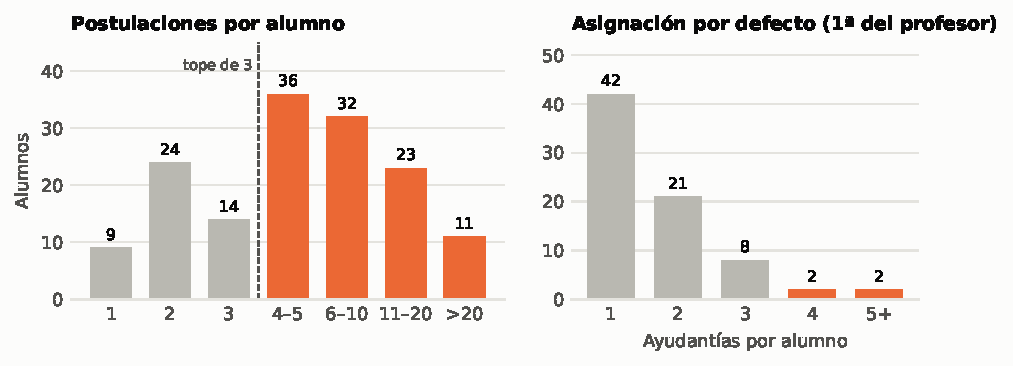
\includegraphics[width=\textwidth]{figuras/situacion_actual.pdf}
\caption{Izquierda: cantidad de postulaciones por alumno; en naranjo, quienes postulan a más ayudantías que el tope. Derecha: ayudantías por alumno si cada unidad tomara a la 1ª prioridad de su profesor; en naranjo, los alumnos sobre el tope, que el Secretario debe corregir a mano.}
\label{fig:situacion}
\end{figure}

De estas cifras se desprenden cuatro observaciones:
\begin{itemize}
    \item \textbf{El conflicto es estructural.} Dos de cada tres postulantes piden más ayudantías de las que pueden recibir, y el 10\,\% que más postula concentra casi el 40\,\% de las postulaciones. Si cada profesor recibiera a su primer candidato, cuatro alumnos quedarían sobre el tope (uno con seis ayudantías).
    \item \textbf{La corrección manual es local.} Cada ``enroque'' resuelve un alumno sobrecargado pero puede crear otro. Solo 75 de los 149 postulantes reciben ayudantía, 14 reciben tres y 42 alumnos que estaban entre los tres primeros de algún profesor quedan sin ninguna.
    \item \textbf{No se controlan los horarios ni la elegibilidad de forma sistemática.} La asignación real tiene 3 alumnos con dos ayudantías en el mismo bloque y \elegHistNo{} asignaciones a alumnos que no cumplen el criterio base de notas.
    \item \textbf{Las decisiones son difíciles de explicar.} 69 postulaciones fueron rechazadas siendo la primera preferencia del profesor, 15 de ellas también la primera del alumno: son exactamente los reclamos que el Secretario relata.
\end{itemize}

\subsection{Dimensiones}

\begin{itemize}
    \item \textbf{Organizacional (alcance espacial):} los cursos CIT de la EIT; las ayudantías en otros departamentos solo restan capacidad al alumno.
    \item \textbf{Temporal:} la decisión se toma una vez por semestre, antes del inicio de clases, y hoy demora alrededor de un día. Dentro de la semana, las actividades ocupan bloques de 80 minutos y cada ayudantía de cátedra o laboratorio ocupa exactamente uno; la corrección no ocupa bloque.
    \item \textbf{Capacidad:} 127 unidades con presupuesto (218 en toda la oferta CIT: 213 unidades SAP y 5 secciones sin par en la oferta, Sección~\ref{sec:unidades}); a lo más 3 ayudantías por alumno.
    \item \textbf{Elegibilidad:} umbral de promedio general y de nota del ramo.
    \item \textbf{Preferencias:} tres órdenes: el del profesor sobre los postulantes, el del alumno sobre sus postulaciones y el orden por notas de la sección.
\end{itemize}

\subsection{Decisiones}

La decisión es la variable binaria $x_{ij} = 1$ si el alumno $i$ ocupa la unidad $j$. De ella se derivan qué unidades quedan sin cubrir, cuántas ayudantías recibe cada alumno, cuántos no elegibles se usan y en qué posición de cada orden queda cada asignación.

\subsection{Supuestos}
\label{sec:supuestos}

\begin{enumerate}
    \item Las postulaciones, los rankings de los profesores y la programación académica son conocidos antes de asignar.
    \item \textbf{Las postulaciones son válidas}: la plataforma ya verifica los requisitos de postulación y no permite enviar una postulación que no califica. El modelo no vuelve a validarlas.
    \item \textbf{El postulante no tiene colisiones con sus propios ramos}; solo se controlan los topes entre ayudantías.
    \item Cada unidad (grupo de ayudantía o laboratorio, Sección~\ref{sec:unidades}) requiere un ayudante por tipo; en el escenario base, solo las 127 unidades que tuvieron ayudante en 2026-2 tienen presupuesto.
    \item Tope de 3 ayudantías por alumno, menos las que tenga en otros departamentos.
    \item El corrector no ocupa bloque horario; cátedra y laboratorio ocupan el bloque de la sesión. Las 5 secciones sin par en la oferta (Sección~\ref{sec:unidades}) sí tienen un horario, pero se desconoce, por lo que sus topes no se controlan.
    \item Si el profesor no rankeó a un postulante, este se ubica después de los rankeados según el orden por defecto (notas).
    \item La elegibilidad se define por umbrales de promedio y nota del ramo que fija el usuario; el dato oficial de elegibilidad puede cargarse a mano en una plantilla.
    \item El sistema propone; la decisión final sigue siendo del Secretario.
\end{enumerate}

% =====================================================================
\section{Objetivos}
\label{sec:objetivos}

\subsection{Objetivo principal}

Entregar al Secretario Académico una herramienta que, a partir de las postulaciones, los rankings y la programación del semestre, calcule en segundos una \textbf{asignación global} que cubra la mayor cantidad posible de unidades con presupuesto sin violar ninguna restricción dura (en el caso de los horarios, entre los bloques conocidos) y que, entre todas las asignaciones de máxima cobertura, sea la que mejor equilibra las preferencias de profesores, alumnos y el mérito académico. El modelo para lograrlo es el flujo máximo de costo mínimo propuesto en la Entrega 1.

\subsection{Objetivos específicos}

\begin{enumerate}
    \item[OE1.] Representar todas las restricciones duras (tope por alumno, cupos, tipo, postulación y topes entre ayudantías) como capacidades de la red, con cero violaciones; en particular, eliminar los topes horarios entre ayudantías mediante la capa $H$, con los correctores en un bloque ficticio. La garantía de cero topes vale entre los bloques horarios conocidos; las unidades con horario desconocido requieren validación manual antes de la asignación definitiva.
    \item[OE2.] Modelar las preferencias como $aP^O + bP^E + cP^A$, con pesos ajustables por el usuario, y proponer valores justificados.
    \item[OE3.] Garantizar que la cobertura sea el criterio primario y la calidad el secundario (objetivo lexicográfico).
    \item[OE4.] Minimizar el uso de postulantes no elegibles para la cobertura alcanzada, considerando conjuntamente las restricciones del sistema, y exportar esos casos para decisión manual. En el modo de dos pasadas es una garantía del método (Sección~\ref{sec:algoritmo}); con la penalización $d$ depende del valor elegido y se verifica experimentalmente (E5).
    \item[OE5.] Medir y comparar cuantitativamente el modelo con el proceso manual y con el ranking independiente por curso.
\end{enumerate}

\subsection{Evaluación de la situación actual frente a los objetivos}

\begin{table}[H]
\centering
\small
\begin{tabularx}{\textwidth}{l >{\raggedright\arraybackslash}X >{\raggedright\arraybackslash}X >{\raggedright\arraybackslash}X}
\toprule
\textbf{Obj.} & \textbf{Indicador} & \textbf{Situación actual (manual, 2026-2)} & \textbf{Meta} \\
\midrule
Principal & Tiempo y forma de obtener la asignación & $\sim$1 día de ajustes en Excel, no reproducible & segundos, reproducible y auditable \\
OE1 & Violaciones de restricciones duras & 0 excesos del tope, 3 topes horarios entre ayudantías & 0 \\
OE2 & Peso explícito de cada actor & implícito: ``la prioridad del alumno pasa a segundo plano'' & $a$, $b$, $c$ explícitos, con su efecto cuantificado \\
OE3 & Cobertura de las 127 unidades & 100\,\% & 100\,\% \\
OE4 & No elegibles asignados & \elegHistNo{}, decididos a mano & solo los necesarios para cubrir, y listados \\
OE5 & Métricas registradas & ninguna & métricas de la §8 de la Entrega 1 \\
\bottomrule
\end{tabularx}
\caption{Situación actual frente a cada objetivo. El resultado alcanzado se resume en la Tabla~\ref{tab:cumplimiento}.}
\label{tab:objetivos}
\end{table}

% =====================================================================
\section{Datos}
\label{sec:datos}

\subsection{Datos disponibles}

Se trabajó con dos fuentes:

\begin{enumerate}
    \item \textbf{Postulaciones anonimizadas} (\texttt{postulaciones\_ayudantias\_anonimo.xlsx}). Una fila por postulación, con: identificador anónimo, sigla, curso, tipo de ayudante, nota del ramo, promedio general, prioridad que el alumno le dio a la postulación, total de postulaciones del alumno, ranking del profesor, cantidad de postulantes en la sección y estado final (elegido o rechazado).
    \item \textbf{Programación académica} (\texttt{Horarios Ing\_inf.xls}), exportada desde SAP. Contiene la oferta completa del semestre: sección, tipo de evento (cátedra, laboratorio, ayudantía obligatoria, inglés), horario y profesor.
\end{enumerate}

\begin{table}[H]
\centering
\small
\begin{tabular}{lr}
\toprule
\textbf{Dato} & \textbf{Valor} \\
\midrule
Postulaciones & 1.245 \\
Postulantes (alumnos) & 149 \\
Cursos con postulaciones & 33 \\
Postulaciones por alumno (media / máx.) & 8,4 / 77 \\
Postulaciones sin ranking del profesor & 69 \\
Secciones reconstruidas & 165 \\
Secciones sin ningún ranking del profesor & 5 \\
Elegidos en el proceso real & 127 \\
Cursos CIT en la oferta & 44 \\
Unidades ofertadas (cátedra / corrector / lab.) & 79 / 96 / 38 \\
\bottomrule
\end{tabular}

\hspace{1cm}
\begin{tabular}{lrr}
\toprule
\textbf{Tipo} & \textbf{Postulaciones} & \textbf{Elegidos} \\
\midrule
Corrector & 812 & 48 \\
Cátedra & 413 & 74 \\
Laboratorio & 20 & 5 \\
\bottomrule
\end{tabular}

\caption{Datos utilizados: resumen general (izquierda) y postulaciones por tipo de ayudante (derecha).}
\label{tab:datos}
\end{table}

\paragraph{Parámetros que no vienen en los datos.} Los pesos de la función de costo, los umbrales de elegibilidad, el dato oficial de elegibilidad y las ayudantías en otros departamentos no están en los archivos entregados. Todos quedaron como \textbf{entrada del usuario} en \texttt{parametros.json} (Anexo~\ref{sec:anexo-param}); para este informe se probaron varios valores y se eligieron los más adecuados (Secciones~\ref{sec:res-pesos} y~\ref{sec:res-elegibilidad}).

\subsection{Reconstrucción de secciones}
\label{sec:reconstruccion}

El archivo anonimizado indica sigla y tipo, pero \textbf{no el número de sección}, y sin sección no es posible definir los cupos ni los bloques horarios. Sin embargo, el archivo sí incluye la cantidad $N$ de postulantes de la sección. Para cada combinación (sigla, tipo, $N$) existen exactamente $k \cdot N$ filas, lo que corresponde a $k$ secciones de $N$ postulantes. Esta regularidad se cumple en los 137 grupos sin excepción.

Las filas se reparten entre las $k$ secciones mediante \textbf{backtracking}, imponiendo tres condiciones: un alumno aparece a lo más una vez por sección; el ranking del profesor no se repite dentro de una sección; y hay a lo más un elegido histórico por sección. Se obtienen 165 secciones. Cuando $k = 1$ la sección es exacta; cuando $k > 1$ el backtracking entrega la primera partición que cumple las condiciones, y puede haber otras. La reconstrucción es, por lo tanto, \emph{factible}, no necesariamente la partición original.

\subsection{Unidades de demanda a partir de la oferta}
\label{sec:unidades}

La programación SAP revela que, en los cursos con laboratorio, \textbf{dos secciones SAP comparten la misma cátedra y la misma ayudantía}. Por ejemplo, CIT2107 tiene 7 secciones de laboratorio y solo 4 grupos de cátedra (eventos ``MADRE''). Por ello, la unidad que demanda un ayudante no es la sección SAP sino:

\begin{table}[H]
\centering
\small
\begin{tabular}{lll}
\toprule
\textbf{Tipo} & \textbf{Unidad (nodo $C_j$)} & \textbf{Bloque que ocupa el ayudante} \\
\midrule
Cátedra & cada evento \textsc{Ayudantía} distinto & el de la ayudantía \\
Corrector & el mismo grupo de la cátedra & bloque ficticio de corrección \\
Laboratorio & cada evento \textsc{Laboratorio} & el del laboratorio \\
\bottomrule
\end{tabular}
\caption{Unidades de demanda derivadas de la programación académica.}
\label{tab:unidades}
\end{table}

Así se obtienen 213 unidades (79 de cátedra, 96 de corrector y 38 de laboratorio). La cantidad de secciones reconstruidas coincide con la de grupos reales en 30 de los 33 cursos con postulaciones, lo que es consistente tanto con la reconstrucción como con esta interpretación. En los tres cursos restantes (CIT2108, CIT2110 y CIT3203) la reconstrucción entrega 5 secciones más que los grupos SAP. Esas secciones no tienen par en la oferta, pero tienen postulantes rankeados, así que se conservan como unidades de demanda, sin bloque conocido. Por eso el escenario de toda la oferta (E2) tiene 218 cupos: las 213 unidades SAP más esas 5.

\paragraph{Supuesto de emparejamiento.} Los datos anonimizados no permiten saber qué sección reconstruida corresponde a qué grupo real dentro de un mismo curso. El emparejamiento se hace al azar con una semilla fija; la Sección~\ref{sec:res-robustez} evalúa su efecto sobre 100 emparejamientos distintos.

\subsection{Orden por defecto y rankings faltantes}
\label{sec:orden-defecto}

Para cada sección se define un \textbf{orden por defecto} de los postulantes: de mayor a menor nota en el ramo y, a igual nota, de mayor a menor promedio general. Este orden cumple dos funciones. Es la tercera preferencia del modelo ($P^A$, mérito en la asignatura). Y completa el ranking del profesor cuando falta: \sinRankPost{} postulaciones no tienen ranking y \sinRankSecciones{} secciones no tienen ninguno. Los no rankeados se ubican \emph{después} de todos los rankeados, en el orden por defecto, de modo que el criterio del profesor siempre prima.

\subsection{Elegibilidad}
\label{sec:elegibilidad}

Se considera \textbf{elegible} la postulación de un alumno con promedio general y nota del ramo sobre los umbrales que fija el usuario (base: \elegPromMin{} y \elegNotaMin; una nota faltante no descalifica). Con el criterio base, \elegPostNo{} de las \elegPostTotal{} postulaciones no son elegibles y \elegAlumNoProm{} alumnos no alcanzan el promedio mínimo. Como el criterio oficial (ranking de la generación, ramos reprobados) no viene en el archivo anonimizado, el prototipo \textbf{exporta una plantilla por alumno} con los criterios básicos calculados y una columna \texttt{elegible\_manual} (SI / NO / vacío) que el Secretario puede completar con el Excel de casa central; si se completa, prima sobre el cálculo.

% =====================================================================
\section{Revisión de literatura y selección del método}
\label{sec:literatura}

La selección del método se hizo en dos niveles: primero el \emph{modelo} (cómo formular el problema) y luego el \emph{algoritmo} (cómo resolver ese modelo).

\subsection{Modelos para la asignación de ayudantes}

\begin{itemize}
    \item \textbf{Matching estable.} Abraham, Irving y Manlove~\cite{abraham2007spa} resuelven el \textit{Student-Project Allocation}: estudiantes, proyectos y profesores con capacidades y preferencias de ambos lados, en tiempo lineal, mediante aceptación diferida. Su criterio es la \emph{estabilidad}, no la cobertura: un matching estable puede dejar cupos vacíos que otra asignación factible sí cubriría, lo que contradice la prioridad del Secretario (``necesito asegurar las ayudantías''). La formulación estándar citada tampoco incorpora directamente las restricciones de incompatibilidad horaria del problema.
    \item \textbf{Programación por metas.} Güler et al.~\cite{guler2015ta} asignan tareas a ayudantes con \textit{goal programming}, separando restricciones duras de metas blandas penalizadas. De este trabajo se adoptó la separación duro/blando: lo duro como capacidad, lo blando como costo.
    \item \textbf{Programación lineal entera.} Qu et al.~\cite{qu2017ta} formulan la asignación de ayudantes como programación lineal entera mixta (MILP); Palma et al.~\cite{palma2025uta} integran la selección de ayudantes con la programación de los tutoriales en un único modelo de optimización, evaluado en un caso universitario real. La programación entera es la formulación más general, pero requiere un solver externo y su relajación lineal no es entera en general.
    \item \textbf{Flujo en redes.} La asignación con capacidades es un caso clásico de flujo de costo mínimo~\cite{ahuja1993}. Su ventaja es que la matriz de restricciones es totalmente unimodular: si las capacidades son enteras, existe una solución óptima entera y los algoritmos combinatorios la encuentran directamente, sin ramificación~\cite{ahuja1993}.
\end{itemize}

La clave para elegir es que, en la EIT, \textbf{los horarios están dados}. A diferencia de Palma et al., no hay que decidir cuándo se dicta cada tutorial, sino solo respetarlos, y cada ayudantía ocupa exactamente un bloque. Con eso, la restricción ``a lo más una ayudantía por bloque'' es una capacidad unitaria en el nodo $H_{i,h}$, y \textbf{todo el problema cabe en una red de flujo}. Se conserva así la integralidad y se puede resolver con un algoritmo polinomial propio, sin solver externo.

\paragraph{Ponderación de varios criterios.} El costo combina tres preferencias con pesos que suman uno. Elegir esos pesos es un problema multicriterio: no existe un punto que sea el mejor para los tres actores a la vez. Se usó la \textbf{programación de compromiso}~\cite{zeleny1982}: cada criterio se normaliza entre su mejor valor alcanzable (punto ideal) y su peor valor observado (anti-ideal), y se elige la ponderación cuya solución queda más cerca del ideal.

\subsection{Algoritmos para flujo máximo de costo mínimo}

Escogido el modelo, la Tabla~\ref{tab:algoritmos} compara los algoritmos clásicos para resolverlo.

\begin{table}[H]
\centering
\small
\begin{tabularx}{\textwidth}{>{\raggedright\arraybackslash}p{3.3cm} >{\raggedright\arraybackslash}X >{\raggedright\arraybackslash}p{3.0cm} >{\raggedright\arraybackslash}X}
\toprule
\textbf{Algoritmo} & \textbf{Idea} & \textbf{Complejidad} & \textbf{Adecuación al problema} \\
\midrule
Húngaro~\cite{kuhn1955} & Asignación 1 a 1 en grafo bipartito & $O(n^3)$ & No representa $k_i > 1$ ni la capa $H$ sin duplicar nodos \\
Cancelación de ciclos~\cite{klein1967} & Parte de un flujo máximo y cancela ciclos de costo negativo & pseudo-polinomial & Requiere calcular antes el flujo máximo; más lento en la práctica \\
Escalamiento de costos~\cite{goldberg1990} & Aproximaciones $\varepsilon$-óptimas sucesivas & polinomial & El más rápido en redes grandes, pero complejo de implementar y auditar \\
Network simplex~\cite{orlin1997} & Simplex especializado en árboles generadores & polinomial (variante de Orlin) & Eficiente, pero requiere manejar degeneración \\
\textbf{Successive Shortest Paths}~\cite{busacker1960,tomizawa1971,edmonds1972} & Ford--Fulkerson aumentando siempre por el camino más barato & $O(F\,|A| \log |V|)$ & $F \le 218$: muy rápido aquí; extiende directamente Ford--Fulkerson; entrega el criterio lexicográfico sin modificar el objetivo \\
\bottomrule
\end{tabularx}
\caption{Algoritmos clásicos para flujo máximo de costo mínimo.}
\label{tab:algoritmos}
\end{table}

Se eligió \textbf{Successive Shortest Paths (SSP)} por tres razones:
\begin{enumerate}
    \item \textbf{Entrega exactamente el objetivo lexicográfico.} Tras cada aumento, el flujo es de costo mínimo para su valor; al terminar es máximo. No hace falta resolver en dos fases ni usar constantes ``Big-M''.
    \item \textbf{El tamaño del problema lo hace eficiente.} Su costo depende del flujo total $F$, acotado por el número de unidades ($\leq 218$). Con unos 600--800 nodos, se resuelve en alrededor de 100 ms en Python puro.
    \item \textbf{Es un algoritmo conocido, auditable y continúa la Entrega 1.} Es Ford--Fulkerson, el algoritmo que la Entrega 1 tomó como base (§6.8), con dos modificaciones clásicas: elegir siempre el camino aumentante de menor costo y calcularlo eficientemente con potenciales (Tabla~\ref{tab:cadena}). Se implementó desde cero en menos de 100 líneas, que se verificaron contra \texttt{networkx}. La modalidad de dos pasadas para no elegibles (Sección~\ref{sec:modos}) solo lo ejecuta dos veces; no requiere un algoritmo nuevo.
\end{enumerate}

% =====================================================================
\section{Modelo implementado}
\label{sec:modelo}

\subsection{Red de flujo}

La Figura~\ref{fig:red} muestra la red sobre un ejemplo pequeño. \textbf{Toda restricción dura es una capacidad y la única arista con costo es $H \to C$} (Sección~\ref{sec:cambios}).

\begin{figure}[H]
\centering
\begin{tikzpicture}[
    >={Stealth[length=2mm]},
    nodo/.style={circle, draw=gris, fill=white, minimum size=7mm, inner sep=0pt, font=\small},
    hnodo/.style={rectangle, rounded corners=2pt, draw=gris, fill=white, minimum height=5.5mm, inner sep=2pt, font=\scriptsize},
    cnodo/.style={rectangle, draw=gris, fill=gris!12, minimum height=6mm, inner sep=2pt, font=\scriptsize, align=center},
    arista/.style={->, draw=gris!80, line width=0.6pt},
    costo/.style={->, draw=flujo, line width=0.8pt},
    etq/.style={font=\scriptsize, fill=white, inner sep=1pt},
    x=1cm, y=1cm]
    \node[nodo] (S) at (0,0) {$S$};
    \node[nodo] (E1) at (2.6,1.5) {$E_1$};
    \node[nodo] (E2) at (2.6,-1.5) {$E_2$};
    \node[hnodo] (H11) at (5.4,2.4) {$H_{1,\text{MI 08:30}}$};
    \node[hnodo] (H12) at (5.4,1.2) {$H_{1,\text{JU 13:00}}$};
    \node[hnodo] (H21) at (5.4,0) {$H_{2,\text{MI 08:30}}$};
    \node[hnodo, dashed] (H2c) at (5.4,-1.6) {$H_{2,\text{corr}}$};
    \node[hnodo, dashed] (H1c) at (5.4,-2.6) {$H_{1,\text{corr}}$};
    \node[cnodo] (C1) at (8.6,2.1) {$C_1$ Cátedra G01\\MI 08:30};
    \node[cnodo] (C2) at (8.6,0.6) {$C_2$ Cátedra G02\\MI 08:30};
    \node[cnodo] (C3) at (8.6,-0.9) {$C_3$ Laboratorio\\JU 13:00};
    \node[cnodo] (C4) at (8.6,-2.4) {$C_4$ Corrector\\sin bloque};
    \node[nodo] (T) at (11.4,0) {$T$};

    \draw[arista] (S) -- node[etq, pos=0.5] {$k_1$} (E1);
    \draw[arista] (S) -- node[etq, pos=0.5] {$k_2$} (E2);
    \draw[arista] (E1) -- node[etq, pos=0.5] {1} (H11);
    \draw[arista] (E1) -- (H12);
    \draw[arista] (E2) -- (H21);
    \draw[arista] (E2) -- node[etq, pos=0.5] {3} (H2c);
    \draw[arista] (E1) to[out=-80, in=180] (H1c);
    \draw[costo] (H11) -- node[etq, pos=0.45] {$c_{11}$} (C1);
    \draw[costo] (H11) -- (C2);
    \draw[costo] (H12) -- (C3);
    \draw[costo] (H21) -- (C1);
    \draw[costo] (H21) -- (C2);
    \draw[costo] (H2c) -- node[etq, pos=0.5] {$c_{24}$} (C4);
    \draw[costo] (H1c) -- (C4);
    \foreach \c in {C1,C2,C3,C4} \draw[arista] (\c) -- (T);
    \node[etq] at (10.1,1.4) {$1 \times q_j$};
\end{tikzpicture}
\caption{Red $S \to E \to H \to C \to T$ en un ejemplo. En gris, aristas de capacidad con costo 0; en azul, las únicas aristas con costo. $E_1$ postula a las dos cátedras, que tienen ayudantía a la misma hora; como $c(E_1, H_{1,\text{MI 08:30}}) = 1$, solo puede tomar una. Los correctores pasan por el bloque ficticio $H_{i,\text{corr}}$, de capacidad 3.}
\label{fig:red}
\end{figure}

Las aristas y sus capacidades son:

\begin{itemize}
    \item \textbf{$S \to E_i$}: capacidad $k_i = \max(0,\, 3 - \text{externas}_i)$ y costo 0; el máximo con 0 evita capacidades negativas si se registran más de tres ayudantías externas. Es el máximo de \emph{adjudicaciones}; las \emph{postulaciones} no tienen límite.
    \item \textbf{$E_i \to H_{i,h}$}: capacidad 1 y costo 0, de modo que hay a lo más una ayudantía por bloque $h$.
    \item \textbf{$E_i \to H_{i,\text{corr}}$}: bloque \textbf{ficticio} de corrección, capacidad $\min(3, k_i)$ y costo 0. La corrección no ocupa un bloque real, así que un alumno puede corregir en varias unidades; con capacidad 1 quedaría limitado a una sola. Por falta de dato, también pasan por este nodo las 5 secciones sin par en la oferta (Sección~\ref{sec:unidades}). No es lo mismo que no tener horario: esas unidades sí tienen uno, pero se desconoce, así que sus topes no se controlan. En el escenario base esto afecta a 3 unidades de cátedra o laboratorio con cupo.
    \item \textbf{$H_{i,h} \to C_j$}: capacidad 1 y costo $c_{ij}$. Existe si el alumno postuló a $C_j$, $C_j$ ocurre en el bloque $h$ y el modo de no elegibles lo permite (Sección~\ref{sec:modos}).
    \item \textbf{$C_j \to T$}: una arista de capacidad 1 y costo 0 \textbf{por cada cupo} de la unidad. Si una unidad necesita varios ayudantes, se crean aristas adicionales.
\end{itemize}

\subsection{Función de costo}

El costo de la arista $H_{i,h} \to C_j$ es una \textbf{combinación convexa} de tres preferencias:
\[
    c_{ij} = a\,P^O_{ij} + b\,P^E_{ij} + c\,P^A_{ij} + d\,[\,i \text{ no elegible para } j\,], \qquad a + b + c + d = 1,\quad a, b, c, d \geq 0.
\]
Cada preferencia es un \textbf{ranking normalizado} a $[0, 1]$, con $0$ para la primera opción y $1$ para la última: si $r$ es la posición y $R$ el largo de la lista, $P = (r - 1)/(R - 1)$, y $P = 0$ si la lista tiene un solo elemento.
\begin{itemize}
    \item $P^O$ (\textbf{oferta}): posición del alumno en el ranking del profesor de la sección, completado con el orden por defecto (Sección~\ref{sec:orden-defecto}).
    \item $P^E$ (\textbf{estudiante}): prioridad que el alumno le dio a la postulación, dentro de todas las suyas.
    \item $P^A$ (\textbf{asignatura}): posición en el orden por defecto de la sección (nota del ramo y promedio).
\end{itemize}
La normalización hace que los tres términos sean comparables: sin ella, un alumno con 77 postulaciones tendría una prioridad 50 que pesaría más que cualquier ranking del profesor. Con $a + b + c + d = 1$, el costo de toda arista está en $[0, 1]$ y los pesos se leen directamente como la importancia relativa de cada actor. Geométricamente, la proporción $a : b : c$ es un punto del triángulo de la Figura~\ref{fig:pesos}, y $d$ fija cuánto pesa la elegibilidad frente a las tres preferencias. Para el algoritmo, los costos se multiplican por 1.000 y se redondean a enteros.

Los pesos se eligieron con dos experimentos: la proporción $a : b : c = \propA : \propB : \propC$ con E4 (Sección~\ref{sec:res-pesos}) y $d = \pesoD$ con E5 (Sección~\ref{sec:res-elegibilidad}), lo que da $a = \pesoA$, $b = \pesoB$, $c = \pesoC$, $d = \pesoD$. Son valores \emph{sintéticos} propuestos para el informe; en la práctica los fija el Secretario en \texttt{parametros.json}.

\subsection{Modos para los postulantes no elegibles}
\label{sec:modos}

Se asume que la plataforma solo deja enviar postulaciones válidas, pero pueden quedar unidades cuyos únicos candidatos no cumplen el criterio de elegibilidad. La relevancia de los no elegibles es configurable, desde no tomarlos en cuenta hasta tratarlos como a cualquier postulante:
\begin{itemize}
    \item \textbf{Excluir} (no se toman en cuenta). Las postulaciones no elegibles no tienen arista; los cupos que quedan vacíos se exportan para decisión manual.
    \item \textbf{Penalizar con $d$} (se toman en cuenta, con relevancia graduable; por defecto). Una sola pasada con todas las aristas; las de no elegibles cuestan $d$ más, con $d$ como cuarto peso de la ponderación ($a + b + c + d = 1$). Como la cobertura es el criterio primario, un no elegible siempre puede entrar si es la única forma de cubrir un cupo. Con $d$ alto (\neDCritico{} o más en los casos evaluados en E5), el número de no elegibles asignados coincide con el mínimo necesario para alcanzar la cobertura obtenida; con $d$ menor, un no elegible muy bien rankeado puede ganarle a un elegible; con $d = 0$ la elegibilidad no tiene efecto.
    \item \textbf{Dos pasadas} (variante estricta). La 1ª pasada resuelve el flujo solo con elegibles; la 2ª, sobre lo que quedó libre (cupos sin cubrir, capacidad restante y bloques no usados), solo con no elegibles. Nunca desplaza a un elegible (Algoritmo~\ref{alg:dos}).
\end{itemize}
En todos los modos, los cupos que quedan vacíos se listan con sus candidatos y el motivo en la hoja \emph{Decisión manual}, para que el Secretario decida.

\begin{algorithm}[H]
\caption{Asignación en dos pasadas}
\label{alg:dos}
\begin{algorithmic}[1]
\Require postulaciones, unidades con cupos, bloques, parámetros
\Ensure asignación $X$
\State $G_1 \gets$ red con solo las aristas de postulaciones \textbf{elegibles}
\State $X_1 \gets \textsc{SSP}(G_1)$ \Comment{flujo máximo de costo mínimo}
\State $G_2 \gets$ red con capacidades residuales: $k_i - |X_1(i)|$, bloques de $X_1$ eliminados, cupos sin cubrir; solo aristas \textbf{no elegibles}
\State $X_2 \gets \textsc{SSP}(G_2)$
\State \Return $X_1 \cup X_2$ \Comment{los cupos que siguen vacíos van a ``Decisión manual''}
\end{algorithmic}
\end{algorithm}

\subsection{Restricciones}

\begin{table}[H]
\centering
\small
\begin{tabular}{lll}
\toprule
\textbf{Restricción} & \textbf{Mecanismo en la red} & \textbf{Tipo} \\
\midrule
Máximo de 3 ayudantías por alumno (menos externas) & $c(S, E_i) = k_i$ & Capacidad \\
Postulación (válida por supuesto) & existencia de la arista hacia $C_j$ & Estructura \\
Cupos por unidad & $q_j$ aristas $C_j \to T$ de capacidad 1 & Capacidad \\
Tipo de ayudantía & cada tipo es un nodo $C_j$ distinto & Estructura \\
Sin topes entre ayudantías & $c(E_i, H_{i,h}) = 1$ & Capacidad \\
Corrección fuera de horario & $c(E_i, H_{i,\text{corr}}) = \min(3, k_i)$ & Capacidad \\
Preferencias de profesor, alumno y asignatura & $aP^O + bP^E + cP^A$ en $H \to C$ & Costo \\
Elegibilidad (por defecto) & $+d$ en $H \to C$ & Costo \\
Elegibilidad (modos estrictos) & segunda pasada / sin arista & Estructura \\
\bottomrule
\end{tabular}
\caption{Restricciones y su representación en la red.}
\label{tab:restricciones}
\end{table}

\subsection{Algoritmo: caminos mínimos sucesivos}
\label{sec:algoritmo}

\subsubsection{Fundamento teórico}

El problema de la Entrega 1 (§6.6) es encontrar, en una red $G = (V, A)$ con capacidades enteras $u \geq 0$ y costos $c$, el flujo $S \to T$ de valor máximo y, entre todos los de valor máximo, el de costo mínimo. Se resolvió con \textbf{Successive Shortest Paths} (SSP, caminos mínimos sucesivos), propuesto por Busacker y Gowen~\cite{busacker1960}: partiendo de $f = 0$, se aumenta repetidamente el flujo por el camino $S \leadsto T$ de \emph{menor costo} en la red residual $G_f$, hasta que $T$ deja de ser alcanzable. Su corrección descansa en tres resultados clásicos~\cite{ahuja1993}:

\begin{enumerate}
    \item[(T1)] \textbf{Optimalidad por ciclos negativos}~\cite{klein1967}. Un flujo de valor $v$ es de costo mínimo entre los de valor $v$ si y solo si $G_f$ no tiene ciclos de costo negativo.
    \item[(T2)] \textbf{Invariante del SSP}~\cite{busacker1960}. Si $f$ es de costo mínimo para su valor y se aumenta por un camino de costo mínimo de $G_f$, el nuevo flujo es de costo mínimo para su nuevo valor. Como $f = 0$ con costos no negativos cumple (T1), la invariante se mantiene en todas las iteraciones.
    \item[(T3)] \textbf{Flujo máximo}~\cite{fordfulkerson1956}. El algoritmo termina cuando no existe camino aumentante, lo que, por el teorema de flujo máximo y corte mínimo, ocurre exactamente cuando $f$ es máximo.
\end{enumerate}

De (T2) y (T3), al terminar $f$ es máximo y de costo mínimo entre los máximos: \textbf{el criterio lexicográfico se obtiene directamente}, sin resolver en dos fases ni usar constantes ``Big-M''. Además, por el \textbf{teorema de integralidad}, si las capacidades son enteras cada aumento es entero y el flujo final también lo es~\cite{ahuja1993}; como cada iteración aumenta al menos una unidad, hay a lo más $F$ iteraciones.

\paragraph{Potenciales.} La red residual contiene aristas inversas de costo $-c$, por lo que en principio el camino mínimo exigiría Bellman--Ford. Tomizawa~\cite{tomizawa1971} y Edmonds y Karp~\cite{edmonds1972} mostraron que basta Dijkstra si se trabaja con costos reducidos $c^\pi(u, v) = c(u, v) + \pi(u) - \pi(v)$ y, tras cada búsqueda, se actualiza $\pi \gets \pi + \text{dist}$ en los nodos alcanzables. Esta actualización mantiene no negativos los costos reducidos de las aristas residuales que pueden explorarse desde la fuente, lo que permite aplicar Dijkstra en cada iteración (las aristas de nodos inalcanzables nunca se vuelven a explorar; Tabla~\ref{tab:adaptacion}). Esta reponderación no cambia cuál es el camino mínimo, porque el costo reducido de un camino $S \leadsto T$ es su costo real más la constante $\pi(S) - \pi(T)$. La complejidad total es $O(F \cdot |A| \log |V|)$.

\begin{algorithm}[H]
\caption{Successive Shortest Paths con potenciales (implementado en \texttt{ayudantias/flujo.py})}
\label{alg:ssp}
\begin{algorithmic}[1]
\Require red $G=(V,A)$ con capacidades enteras $u$ y costos enteros $c \geq 0$; fuente $S$, sumidero $T$
\Ensure flujo $f$ máximo y de costo mínimo entre los flujos máximos
\State $f \gets 0$; \quad $\pi(v) \gets 0 \ \ \forall v \in V$
\Loop
    \State calcular con Dijkstra la distancia $d(v)$ desde $S$ en $G_f$ con costos reducidos $c^\pi(u,v) = c(u,v) + \pi(u) - \pi(v)$
    \If{$T$ no es alcanzable} \textbf{terminar} \EndIf
    \State $\pi(v) \gets \pi(v) + d(v)$ para todo $v$ alcanzable
    \State $P \gets$ camino de costo mínimo $S \leadsto T$; \quad $\delta \gets \min_{(u,v) \in P} u_f(u,v)$
    \State aumentar $f$ en $\delta$ a lo largo de $P$ (y descontar en las aristas residuales)
\EndLoop
\State \Return $f$
\end{algorithmic}
\end{algorithm}

\subsubsection{Del algoritmo base a la versión implementada}

El algoritmo implementado no es nuevo: es Ford--Fulkerson, la base de la Entrega 1 (§6.8), con dos modificaciones conocidas de la literatura y un conjunto de adaptaciones de modelado al caso de la EIT. La Tabla~\ref{tab:cadena} muestra cada paso, qué cambia respecto del anterior, qué garantiza y en qué trabajo se sustenta.

\begin{table}[H]
\centering
\small
\begin{tabularx}{\textwidth}{>{\raggedright\arraybackslash}p{3.2cm} >{\raggedright\arraybackslash}X >{\raggedright\arraybackslash}X}
\toprule
\textbf{Paso} & \textbf{Qué cambia} & \textbf{Qué garantiza} \\
\midrule
0. Ford--Fulkerson~\cite{fordfulkerson1956} & Aumenta el flujo por \emph{cualquier} camino $S \leadsto T$ de la red residual & Flujo máximo (T3), pero ignora los costos: cubre lo máximo sin mirar preferencias \\
1. Successive Shortest Paths~\cite{busacker1960} & Aumenta siempre por el camino de \emph{menor costo} & Cada flujo intermedio es de costo mínimo para su valor (T2, sustentada en T1~\cite{klein1967}); al terminar, el óptimo lexicográfico \\
2. Potenciales~\cite{tomizawa1971,edmonds1972} & Busca el camino con Dijkstra sobre costos reducidos, en vez de Bellman--Ford & El mismo camino mínimo, en $O(|A| \log |V|)$ por iteración \\
3. Adaptación al caso~\cite{ahuja1993} & Capa $H$ por división de nodos, bloque ficticio, aristas paralelas por cupo, costos enteros y tratamiento de no elegibles & La red sigue siendo de flujo ordinaria con capacidades enteras: T1--T3 e integralidad se conservan (Tabla~\ref{tab:adaptacion}) \\
\bottomrule
\end{tabularx}
\caption{Del algoritmo de la Entrega 1 al implementado.}
\label{tab:cadena}
\end{table}

\subsubsection{Adaptación al problema y garantías que se conservan}

La Tabla~\ref{tab:adaptacion} detalla el paso 3: muestra cómo se llevó el problema de asignación a la forma que el SSP resuelve, y por qué cada adaptación conserva (T1)--(T3) y la integralidad.

\begin{table}[H]
\centering
\small
\begin{tabularx}{\textwidth}{>{\raggedright\arraybackslash}p{4.2cm} >{\raggedright\arraybackslash}X}
\toprule
\textbf{Adaptación} & \textbf{Qué se conserva y por qué} \\
\midrule
La asignación $x_{ij} \in \{0,1\}$ es el flujo en la arista $H \to C$ & Todas las capacidades son enteras: por integralidad, el óptimo es 0/1 sin programación entera \\
Una ayudantía por bloque: nodo $H_{i,h}$ con una sola arista de entrada de capacidad 1 & Es la técnica estándar de dividir un nodo para imponerle capacidad; la red sigue siendo de flujo ordinaria \\
Bloque ficticio de corrección con capacidad $\min(3, k_i)$ & Es una arista más con capacidad entera \\
Varios cupos como aristas paralelas $C_j \to T$ & Las aristas se almacenan como lista, de modo que las paralelas son legítimas; con costo 0 equivalen a una arista de capacidad $q_j$ \\
Costos en $[0, 1]$, escalados a enteros: $\operatorname{round}(1000\, c_{ij})$ & Costos enteros y no negativos: se cumplen las hipótesis de (T1)--(T3) y de los potenciales. El redondeo evita errores de punto flotante en Dijkstra y aleja el costo del óptimo real en a lo más $F \times 0{,}001$, en la escala original del costo, $[0, 1]$; la cobertura no depende de los costos \\
Potenciales actualizados solo en nodos alcanzables & Un nodo que deja de ser alcanzable desde $S$ no vuelve a serlo (las aristas residuales nuevas aparecen solo en el camino aumentado, entre nodos alcanzables), así que sus aristas no se vuelven a examinar \\
Elegibilidad, modo excluir: se eliminan aristas & SSP sobre un subgrafo: (T1)--(T3) valen sin cambios \\
Elegibilidad, modo penalizar: $+d$ en el costo & Los costos siguen no negativos: (T1)--(T3) valen sin cambios \\
\bottomrule
\end{tabularx}
\caption{Adaptaciones del SSP al problema de asignación.}
\label{tab:adaptacion}
\end{table}

\subsubsection{Garantías en los dos tratamientos de los no elegibles}

\paragraph{Una pasada con penalización $d$ (por defecto).} Es un único SSP sobre la red completa, por lo que se aplican (T1)--(T3) directamente: la solución tiene \textbf{la máxima cobertura posible} con todos los postulantes y, entre las de máxima cobertura, el menor costo. El peso $d$ solo actúa en el segundo criterio: decide entre asignaciones con la misma cobertura y \textbf{nunca sacrifica un cupo}. Un no elegible entra si es la única forma de cubrir un cupo o, cuando $d$ es pequeño, si su ventaja en las preferencias supera la penalización. Como el SSP puede reasignar a lo largo de un camino aumentante, un elegible puede moverse a otra unidad para dejar espacio a un no elegible si eso aumenta la cobertura.

\paragraph{Dos pasadas (variante estricta, Algoritmo~\ref{alg:dos}).} Son dos SSP consecutivos. La primera pasada, sobre la red con solo aristas elegibles, entrega por (T1)--(T3) la \textbf{máxima cobertura alcanzable solo con elegibles}, al menor costo. La segunda pasada, sobre las capacidades residuales y solo con aristas no elegibles, entrega la máxima cobertura \emph{adicional}, al menor costo, \textbf{sin modificar} la primera. El procedimiento prioriza la máxima cobertura con elegibles y, manteniendo fija la asignación obtenida, maximiza la cobertura adicional con no elegibles. No es un óptimo lexicográfico completo: no garantiza la máxima cobertura total entre todas las soluciones que alcanzan la máxima cobertura con elegibles. Por ejemplo, si el alumno A (elegible) postula a las unidades 1 y 2 y el alumno B (no elegible) solo a la 1, la primera pasada puede asignar A a la unidad 1, con lo que B queda fuera y se cubre una unidad; la asignación de A a la 2 y de B a la 1 tiene la misma cobertura con elegibles y cubre dos. De aquí se siguen dos propiedades:
\begin{itemize}
    \item para la cobertura $C$ que alcanza, usa el \textbf{mínimo número posible de no elegibles}. Sea $M_e$ la cobertura de la primera pasada. Si en cualquier asignación factible se conservan solo sus asignaciones de elegibles, lo que queda es un flujo factible de la red de la primera pasada, así que cubre a lo más $M_e$ unidades. Por lo tanto, toda asignación que cubre $C$ cupos usa al menos $C - M_e$ no elegibles. Las dos pasadas usan exactamente $C - M_e$, y ninguna reorganización de los elegibles puede bajar esa cota;
    \item \textbf{no garantiza la máxima cobertura total}: como la segunda pasada no puede reasignar a los elegibles ya fijados, puede existir una asignación con más cupos cubiertos que requiera mover a un elegible para hacer espacio a un no elegible.
\end{itemize}
En los datos de 2026-2 ambas variantes alcanzan la misma cobertura total en los tres escenarios (Tabla~\ref{tab:lexico}) y usan la misma cantidad de no elegibles cuando $d \geq \neDCritico$ (E5). Sin embargo, la igualdad de cobertura es un resultado empírico de estos datos y no una propiedad del método. Por eso se usa por defecto la penalización, que conserva la garantía de cobertura máxima, y las dos pasadas quedan como alternativa para quien prefiera priorizar a los elegibles por sobre la cobertura.

\subsubsection{Verificación y desempeño}

\begin{itemize}
    \item \textbf{Contra una implementación de referencia.} En cinco ponderaciones aleatorias, con y sin capa horaria, el flujo y el costo coinciden exactamente con \texttt{networkx.max\_flow\_min\_cost}, que usa un algoritmo distinto (network simplex).
    \item \textbf{Criterio lexicográfico.} En los tres escenarios de cupos, el flujo del SSP es igual al flujo máximo calculado sin costos (E6).
    \item \textbf{Optimalidad global.} El ejemplo de la Entrega 1 (§6.9) entrega la asignación de valor 184 y no la local de 125.
    \item \textbf{Desempeño.} En el escenario base la red tiene \redNodos{} nodos y \redAristas{} aristas, con $F = 127$, y se resuelve en unos \redMs{} ms en Python puro.
\end{itemize}
Estas pruebas verifican que la implementación resuelve correctamente el modelo bajo los supuestos declarados. No validan la reconstrucción de los datos ni las reglas institucionales, que se sustentan en la Sección~\ref{sec:datos} y en el levantamiento con el Secretario.

% =====================================================================
\section{Cambios respecto de la Entrega 1}
\label{sec:cambios}

La estructura del modelo se mantiene: red $S \to E \to H \to C \to T$, capacidades para las restricciones duras, costos para las preferencias y objetivo lexicográfico (primero cobertura, después preferencias). Lo que cambió es la \textbf{dirección del diseño}: se adoptó el principio de que \emph{toda regla institucional es una capacidad o parte de la estructura de la red y el único costo es la preferencia de adjudicación}, y se precisaron los elementos que la Entrega 1 dejaba abiertos a partir del levantamiento del proceso (Sección~\ref{sec:levantamiento}), la forma real de los datos (Sección~\ref{sec:datos}) y la evidencia experimental (Sección~\ref{sec:resultados}). La Tabla~\ref{tab:cambios} resume los cambios y a continuación se justifica cada uno.

\begin{table}[H]
\centering
\small
\begin{tabularx}{\textwidth}{>{\raggedright\arraybackslash}p{2.5cm} >{\raggedright\arraybackslash}X >{\raggedright\arraybackslash}X l}
\toprule
\textbf{Elemento} & \textbf{Entrega 1} & \textbf{Entrega 2} & \textbf{Evidencia} \\
\midrule
Usuario, problema, objetivos & genéricos, sin cifras & reescritos con la entrevista y los datos 2026-2 & §\ref{sec:usuario}--\ref{sec:objetivos} \\
Literatura & descriptiva & justifica modelo, algoritmo y elección de pesos & §\ref{sec:literatura} \\
Algoritmo & Ford--Fulkerson; ``extender hacia MCMF'' & Successive Shortest Paths propio & E6, pruebas \\
Principio de diseño & duras en capacidades, blandas en costos (varios costos posibles) & duras en capacidades; \textbf{un solo costo}, en $H \to C$ & pruebas \\
Arista $S \to E_i$ & $c = k_i$ & $c = \max(0,\, 3 - \text{externas}_i)$, costo 0 & E7 \\
Capa $H$ & bloques en que el alumno está disponible & bloques de sus postulaciones + bloque ficticio de corrección & E7 \\
Nodo $C_j$ & ``curso, sección o cupo'' & grupo de ayudantía o laboratorio; una arista a $T$ por cupo & §\ref{sec:unidades} \\
Costo & $\alpha P^E + \beta P^P$, sin definir & $aP^O + bP^E + cP^A + d\,[\text{no eleg.}]$, rankings normalizados, suma 1 & E4, E5 \\
Elegibilidad & restricción dura & excluir, o considerar con relevancia graduable ($d$) & E5 \\
Ranking faltante & no previsto & orden por defecto por notas & E7 \\
Restricciones blandas & preferencias, experiencia, rendimiento, afinidad, distribución & preferencias del profesor y del alumno, rendimiento ($P^A$); distribución como capacidad & E4, E7 \\
Secciones & conocidas & reconstruidas desde los datos & §\ref{sec:reconstruccion} \\
Robustez & -- & análisis sobre 100 emparejamientos & E3 \\
\bottomrule
\end{tabularx}
\caption{Resumen de cambios respecto de la Entrega 1.}
\label{tab:cambios}
\end{table}

\subsection{Usuario, problema, objetivos y literatura}
En la Entrega 1 estas secciones se escribieron antes de conocer el proceso y los datos. En esta entrega se reescribieron con la entrevista y los datos de 2026-2: el usuario incluye su entorno real y una tabla de actores con evidencia; el problema se sustenta en indicadores calculados (Tabla~\ref{tab:situacion}); los objetivos declaran un objetivo principal y se evalúan frente al proceso manual real (Tabla~\ref{tab:objetivos}); y la revisión de literatura se usa para justificar el modelo, el algoritmo y el método para elegir los pesos.

\subsection{Algoritmo}
La Entrega 1 mencionaba Ford--Fulkerson como base y la necesidad de extenderlo a flujo de costo mínimo, sin escoger un algoritmo. Se eligió \textit{Successive Shortest Paths} porque es precisamente esa extensión, un algoritmo clásico y conocido, y porque su invariante garantiza el criterio lexicográfico sin modificar el objetivo (Sección~\ref{sec:literatura}). Se implementó desde cero y se verificó contra \texttt{networkx}.

\subsection{Un solo costo: toda regla institucional es una capacidad}
La Entrega 1 representaba las restricciones duras con capacidades y dejaba abierto representar con costos varias restricciones blandas, entre ellas la ``distribución equilibrada de las ayudantías''. En esta entrega se adoptó un principio más estricto: \textbf{lo que es una regla} (máximo de ayudantías, una ayudantía por bloque, cupos, corrección fuera de horario) \textbf{es una capacidad}, y \textbf{lo que es una preferencia} es el único costo, en la arista de postulación $H \to C$. Todas las demás aristas tienen costo 0.

\emph{Justificación.} Una regla expresada como capacidad no puede violarse ni ``negociarse'' contra una preferencia, y es fácil de explicar a profesores y alumnos (``nadie recibe más de 3''). Un costo en otra arista mezclaría reglas con preferencias y haría que el resultado dependiera de calibrar constantes sin respaldo en los datos. Se consideró la alternativa de repartir ayudantías con costos crecientes en $S \to E_i$, y se descartó: el reparto es una regla institucional (``ojalá que todos tengan 2'') y se logra directamente con la capacidad. El experimento E7 muestra que con $c(S, E_i) = 2$ se cubren igual los 127 cupos y la asignación se reparte entre \capDosAlumnos{} alumnos, sin nadie con 3; con la norma vigente de 3, entre \fAlumnos.

\subsection{Capacidades de la red}
\begin{itemize}
    \item \textbf{$S \to E_i$}: se mantiene $c = k_i$, ahora con $k_i = \max(0,\, 3 - \text{externas}_i)$. El 3 es la norma del Secretario (``estoy utilizando la norma de entregar solamente 3'') y las ayudantías en otros departamentos lo reducen (``ya tomó tres ayudantías en Ciencias Básicas''). Las postulaciones no tienen límite.
    \item \textbf{Bloque ficticio de corrección}: la Entrega 1 suponía que toda ayudantía ocupa un bloque, pero el corrector trabaja fuera de horario. En lugar de conectar el corrector directamente desde $E_i$, se creó un nodo $H_{i,\text{corr}}$ de capacidad $\min(3, k_i)$, de modo que toda arista de postulación sale de la capa $H$ y la corrección no compite por un bloque real. Con capacidad 1 se perderían unidades en toda la oferta (\capCorrUnoOf{} en lugar de \capBaseOf, E7).
    \item \textbf{$C_j \to T$}: la Entrega 1 dejaba abierto si $C$ era un curso, una sección o un cupo. La programación real mostró que en cursos con laboratorio dos secciones SAP comparten la ayudantía (Sección~\ref{sec:unidades}); usar la sección SAP habría duplicado la demanda de cátedra en siete cursos. La unidad es el grupo de ayudantía o laboratorio, y si requiere varios ayudantes se crea una arista de capacidad 1 por cupo.
\end{itemize}

\subsection{Disponibilidad horaria}
La Entrega 1 creaba $H_{i,h}$ solo en los bloques en que el alumno está disponible, lo que exige conocer su inscripción de cursos. Ese dato no existe en el sistema actual (la plataforma de postulación todavía no lo integra) y no fue entregado. Se optó por suponer que el postulante no tiene topes con sus propios ramos y controlar solo los topes entre ayudantías, que sí se conocen a partir de la programación. Modelar la inscripción habría requerido simularla, y los resultados habrían dependido de datos inventados. La red queda preparada: cuando el dato exista, basta con no crear los nodos $H_{i,h}$ ocupados.

\subsection{Función de costo}
La Entrega 1 proponía $c_{ij} = \alpha P^E_{ij} + \beta P^P_{ij}$ sin definir las penalizaciones. En esta entrega:
\begin{itemize}
    \item se agregó una \textbf{tercera preferencia}, $P^A$, el orden de la sección por nota del ramo y promedio, porque son los datos que el Secretario dice mirar (``la nota de asignatura, el promedio en carrera, el ranking [...] y la prioridad del alumno'') y corresponden al ``rendimiento académico'' que la Entrega 1 listaba como restricción blanda;
    \item las tres preferencias se definieron como \textbf{rankings normalizados} a $[0, 1]$, para que sean comparables: sin normalizar, la prioridad 50 de un alumno con 77 postulaciones pesaría más que cualquier ranking del profesor;
    \item los pesos se restringieron a \textbf{sumar 1}, de modo que se leen como la importancia relativa de cada actor y se pueden explorar sistemáticamente sobre un triángulo (E4);
    \item la notación cambió de $\alpha, \beta$ a $a, b, c$ (y $d$, Sección~\ref{sec:modos}), una letra por actor: oferta, estudiante, asignatura.
\end{itemize}
Las otras restricciones blandas de la Entrega 1 (experiencia previa y afinidad de carrera) no se incluyeron porque no están en los datos; pueden agregarse como un término más con el mismo formato.

\subsection{Elegibilidad}
La Entrega 1 trataba la elegibilidad como restricción dura. El levantamiento mostró que en la práctica no lo es: cuando una unidad no tiene candidatos elegibles, el Secretario acepta a uno que no lo es (``tenía tres no elegibles, [...] pa' adentro un no elegible''), pero si hay un elegible, lo prefiere. Por eso se volvió \textbf{graduable}: un valor que no toma en cuenta a los no elegibles (modo excluir, con los cupos vacíos exportados para decisión manual) y valores que sí los toman en cuenta con distinta relevancia, mediante el peso $d$ de la misma ponderación. E5 muestra el efecto de cada nivel y que, desde $d = \neDCritico$, en todos los casos evaluados no se usaron más no elegibles que los necesarios para alcanzar la cobertura obtenida. Además, se asume que la plataforma ya verifica la validez de las postulaciones, por lo que el modelo no la vuelve a revisar.

\subsection{Rankings faltantes}
La Entrega 1 suponía que todo postulante estaba rankeado por su profesor. En los datos, \sinRankPost{} postulaciones no tienen ranking y \sinRankSecciones{} secciones no tienen ninguno. Esos postulantes se ubican después de los rankeados, en el orden por defecto por notas, lo que respeta siempre el criterio del profesor y permite cubrir unidades que de otro modo quedarían vacías (en toda la oferta, \capBaseOf{} frente a \capSinRankOf, E7).

\subsection{Reconstrucción de secciones y análisis de robustez}
Ambos son elementos metodológicos nuevos, exigidos por la forma de los datos anonimizados, que no traen el número de sección. La reconstrucción hace posible el modelo y el análisis de robustez evalúa la sensibilidad frente a uno de los supuestos de reconstrucción: el emparejamiento entre las secciones reconstruidas y los grupos reales (E3).

% =====================================================================
\section{Prototipo}
\label{sec:prototipo}

El prototipo es un programa en Python que lee los mismos archivos que hoy maneja la Secretaría (el Excel de postulaciones y la programación exportada de SAP) más el archivo de parámetros, y produce una planilla Excel con la asignación propuesta. Las 31 pruebas automáticas verifican, entre otras cosas:
\begin{itemize}
    \item el ejemplo de optimización global de la Entrega 1 (§6.9): el modelo encuentra la asignación de valor 184 y no la local de 125;
    \item la equivalencia con \texttt{networkx} en cinco ponderaciones aleatorias;
    \item que la única arista con costo sea $H \to C$;
    \item el cumplimiento de todas las restricciones duras sobre los datos reales;
    \item el bloque ficticio de corrección, los cupos múltiples, el orden por defecto y los modos de no elegibles (en particular, que con $d$ alto se use el mínimo de no elegibles y que la segunda pasada no desplace elegibles);
    \item la validación de \texttt{parametros.json} ($a + b + c + d = 1$, pesos no negativos, modos válidos).
\end{itemize}

\begin{table}[H]
\centering
\small
\begin{tabular}{ll}
\toprule
\textbf{Módulo} & \textbf{Responsabilidad} \\
\midrule
\texttt{parametros.json} & Parámetros que fija el usuario (pesos, capacidades, elegibilidad, externas) \\
\texttt{ayudantias/config.py} & Lectura y validación de los parámetros \\
\texttt{ayudantias/flujo.py} & Successive Shortest Paths (algoritmo propio) \\
\texttt{ayudantias/datos.py} & Postulaciones, reconstrucción de secciones, oferta SAP \\
\texttt{ayudantias/costos.py} & Rankings normalizados, orden por defecto, elegibilidad, costo \\
\texttt{ayudantias/modelo.py} & Red, modos de no elegibles, greedy, decisión manual \\
\texttt{ayudantias/metricas.py} & Métricas de evaluación \\
\texttt{ayudantias/robustez.py} & Análisis sobre múltiples emparejamientos \\
\texttt{main.py} & Ejecución para la Secretaría (salida en Excel, plantilla de elegibilidad) \\
\texttt{experimentos.py} & Experimentos E1--E7 \\
\bottomrule
\end{tabular}
\caption{Módulos del sistema.}
\label{tab:modulos}
\end{table}

\paragraph{Uso por parte del Secretario.} Un ciclo de uso consiste en:
\begin{enumerate}
    \item exportar las postulaciones con el ranking de los profesores y la programación del semestre;
    \item opcionalmente, generar la plantilla de elegibilidad (\texttt{python main.py --exportar-elegibilidad}), completar la columna \texttt{elegible\_manual} con el Excel de casa central y apuntarla en \texttt{parametros.json};
    \item fijar en \texttt{parametros.json} los pesos $a$, $b$, $c$, $d$, el tope, los umbrales y las ayudantías en Ciencias Básicas;
    \item ejecutar \texttt{main.py} y revisar \texttt{salidas/asignacion.xlsx}, en particular la hoja \emph{Decisión manual}.
\end{enumerate}
La planilla trae la asignación (con unidad, bloque, profesor y elegibilidad), la comparación con el proceso manual y el greedy, los cupos sin cubrir con sus candidatos, la elegibilidad por postulación y por alumno, la carga por alumno y los parámetros usados. Mantiene el formato con el que ya trabaja el Secretario y deja la decisión final en sus manos, como establece el alcance de la Entrega 1 (§4.4). Como cada ejecución registra sus parámetros, la asignación puede explicarse a profesores y alumnos, que es la transparencia que pide la encuesta.

% =====================================================================
\section{Resultados}
\label{sec:resultados}

Se comparan tres métodos, identificados con el mismo color en todas las figuras:
\begin{itemize}
    \item \textcolor{manual}{\rule{8pt}{8pt}} \textbf{Manual}: la asignación real del semestre (columna ``Estado'').
    \item \textcolor{greedy}{\rule{8pt}{8pt}} \textbf{Greedy}: cada unidad, por separado, toma al mejor del ranking del profesor que aún tenga capacidad y el bloque libre, prefiriendo elegibles. Emula la Alternativa 1 de la Entrega 1.
    \item \textcolor{flujo}{\rule{8pt}{8pt}} \textbf{Flujo}: el modelo propuesto, con $a/b/c/d = \pesoA/\pesoB/\pesoC/\pesoD$.
\end{itemize}

Salvo indicación, el escenario base usa los cupos que tuvieron ayudante en el semestre (127 unidades), los horarios reales, el emparejamiento con semilla 0 y el criterio de elegibilidad base. Los tres métodos se evalúan con la misma función de costo.

\subsection{E1: Comparación principal}

\begin{figure}[H]
\centering
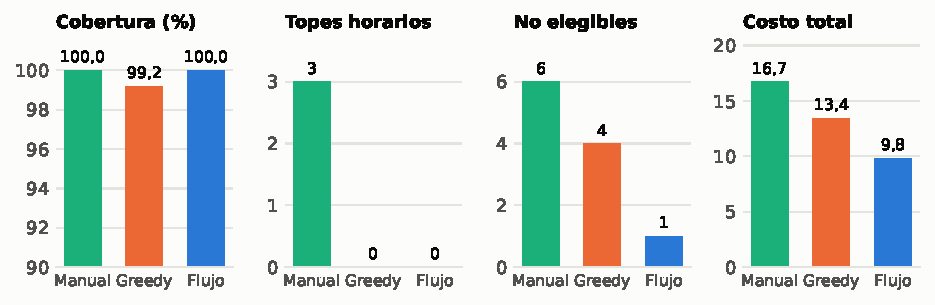
\includegraphics[width=\textwidth]{figuras/metricas_clave.pdf}
\caption{Indicadores principales del escenario base.}
\label{fig:metricas}
\end{figure}

\begin{table}[H]
\centering
\small
\begin{tabular}{lrrr}
\toprule
\textbf{Métrica} & \textbf{Manual} & \textbf{Greedy} & \textbf{Flujo} \\
\midrule
Cupos cubiertos & 127 & 126 & 127 \\
Cobertura & 100,0 \% & 99,2 \% & 100,0 \% \\
Alumnos con ayudantía & 75 & 77 & 77 \\
Alumnos con 1 & 37 & 42 & 43 \\
Alumnos con 2 & 24 & 21 & 18 \\
Alumnos con 3 & 14 & 14 & 16 \\
Excesos del tope de 3 & 0 & 0 & 0 \\
Topes horarios entre ayudantías & 3 & 0 & 0 \\
No elegibles asignados & 6 & 4 & 1 \\
1ª prioridad del profesor & 71,7 \% & 89,7 \% & 63,0 \% \\
Dentro de los 3 primeros del profesor & 97,6 \% & 99,2 \% & 96,9 \% \\
1ª prioridad del alumno & 34,6 \% & 33,3 \% & 39,4 \% \\
Prioridad promedio del alumno & 5,18 & 4,75 & 3,67 \\
1° de la sección por notas & 26,0 \% & 30,2 \% & 41,7 \% \\
$\bar P^O$ (profesor) & 0,113 & 0,057 & 0,097 \\
$\bar P^E$ (estudiante) & 0,354 & 0,335 & 0,245 \\
$\bar P^A$ (asignatura) & 0,356 & 0,318 & 0,230 \\
Costo total (misma función) & 16,73 & 13,42 & 9,83 \\
\bottomrule
\end{tabular}

\caption{Métricas del escenario base. $\bar P^O$, $\bar P^E$ y $\bar P^A$ son la penalización media de cada actor (0 = todos reciben su primera opción). El costo del proceso manual es una evaluación de sus preferencias con la misma función, no una solución factible del modelo: tiene \hChoques{} topes horarios.}
\label{tab:comparacion}
\end{table}

El flujo cubre los 127 cupos, igual que el proceso manual (el greedy deja \gCubiertos{} cubiertos). Además:
\begin{itemize}
    \item \textbf{No hay topes horarios}, frente a \hChoques{} del proceso manual.
    \item \textbf{Usa \fNoEleg{} no elegible}, frente a \hNoEleg{} del manual y \gNoEleg{} del greedy, en una unidad en la que ninguno de sus postulantes es elegible: es el mínimo posible (E5).
    \item \textbf{Mejora a los alumnos y al mérito}: la prioridad promedio que obtiene el alumno baja de \hPromAlum{} a \fPromAlum, y la proporción de asignados que son los primeros de su sección por notas sube de \hNotas\,\% a \fNotas\,\%.
    \item \textbf{Cede algo de la primera preferencia del profesor} (\fPrimProf\,\% frente a \hPrimProf\,\%), aunque el \fTresProf\,\% de las asignaciones queda entre sus tres primeros. Es el resultado de dar peso a los tres actores; la Sección~\ref{sec:res-pesos} muestra cómo se mueve este equilibrio.
\end{itemize}

La Figura~\ref{fig:actores} resume el equilibrio: el flujo consigue las menores penalizaciones para el estudiante y la asignatura, manteniendo la del profesor por debajo de la del proceso manual. A diferencia del greedy, además alcanza la cobertura completa de las 127 unidades.

\begin{figure}[H]
\centering
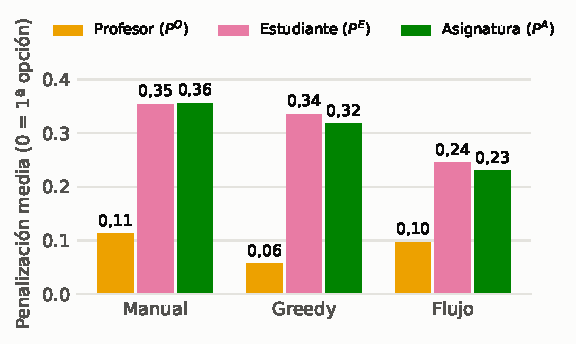
\includegraphics[width=0.66\textwidth]{figuras/actores.pdf}
\caption{Penalización media de cada actor por método (más bajo es mejor).}
\label{fig:actores}
\end{figure}

\begin{figure}[H]
\centering
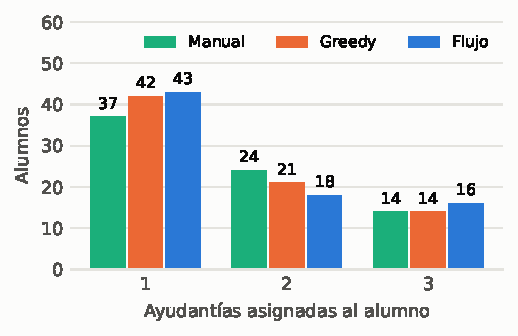
\includegraphics[width=0.6\textwidth]{figuras/carga_alumnos.pdf}
\caption{Cantidad de alumnos según el número de ayudantías asignadas.}
\label{fig:carga}
\end{figure}

La distribución de carga (Figura~\ref{fig:carga}) es parecida en los tres métodos: sin costos de carga, el reparto lo controla solo el tope de 3. El experimento E7 muestra el efecto de cambiarlo.

\begin{figure}[H]
\centering
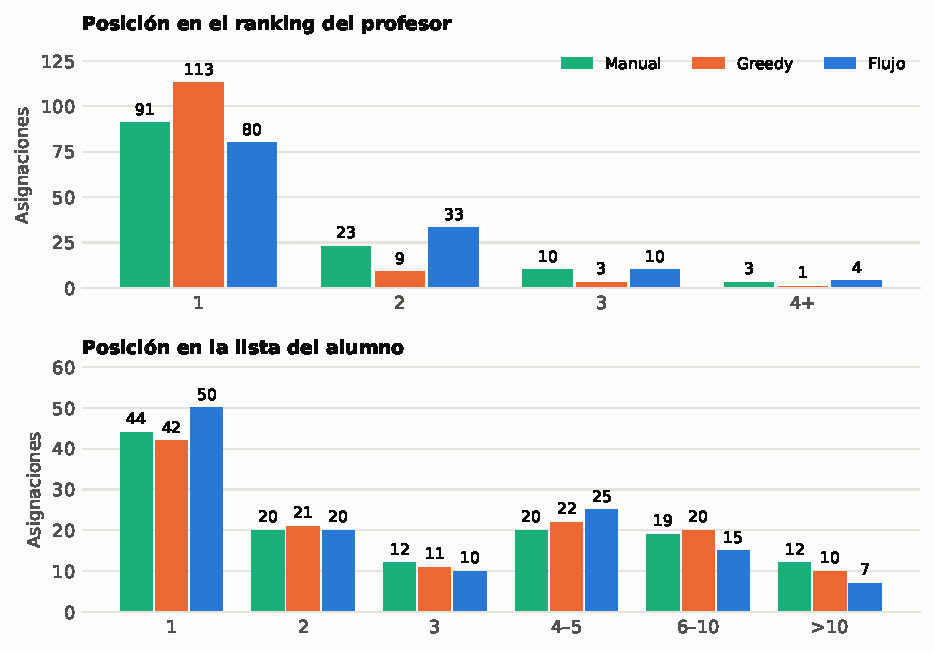
\includegraphics[width=\textwidth]{figuras/prioridades.pdf}
\caption{Distribución de las asignaciones según la posición en el ranking del profesor (arriba, completado con el orden por defecto) y en la lista de preferencias del alumno (abajo).}
\label{fig:prioridades}
\end{figure}

\subsection{La solución vista como grafo}

La Figura~\ref{fig:grafo} muestra el subgrafo de la ayudantía de cátedra de \casoSigla, el curso con postulaciones a cátedra donde más difieren el proceso manual y el flujo. Cada línea es una arista de postulación; las gruesas llevan flujo. Junto a cada alumno se indica cuántas ayudantías recibe en \emph{todo} el proceso.

\begin{figure}[H]
\centering
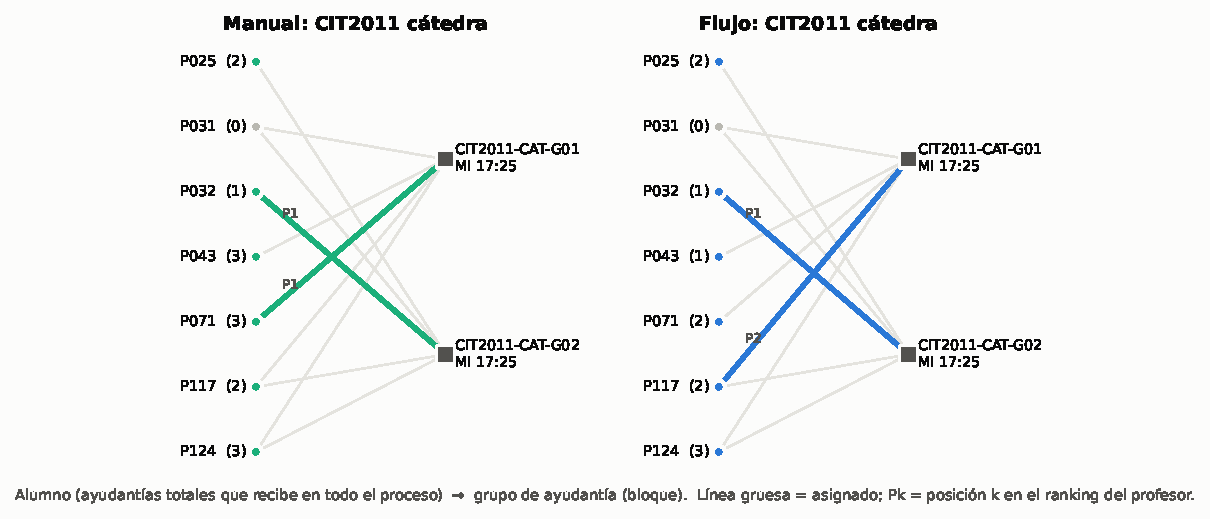
\includegraphics[width=\textwidth]{figuras/solucion_grafo.pdf}
\caption{Solución para la cátedra de \casoSigla. El proceso manual da el grupo G01 a P071, primero del profesor, que termina con tres ayudantías. El flujo se lo da a P117, segundo del profesor, y P071 queda con dos. Los bloques horarios corresponden al emparejamiento de la semilla 0.}
\label{fig:grafo}
\end{figure}

El caso ilustra el argumento de la §6.9 de la Entrega 1 con datos reales: decidir \casoSigla{} de forma aislada no permite ver que el mismo alumno estaba comprometido en otros cursos. El flujo resuelve todos los cursos a la vez.

\begin{figure}[H]
\centering
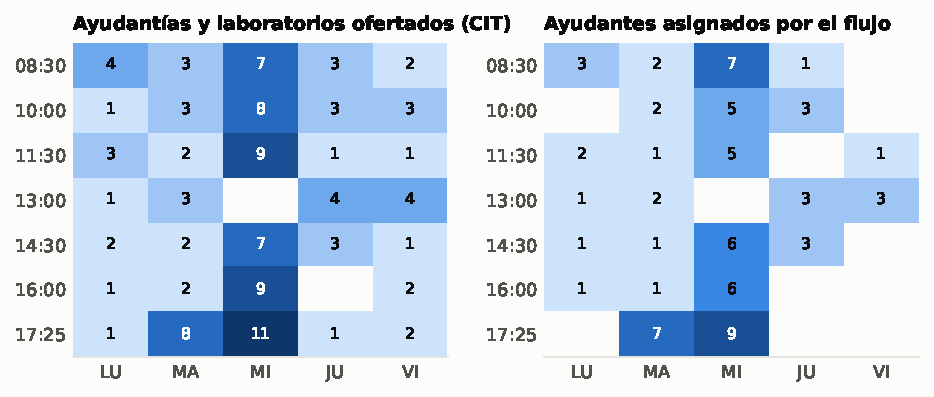
\includegraphics[width=\textwidth]{figuras/horario.pdf}
\caption{Ayudantías y laboratorios ofertados por bloque (izquierda) y ayudantes con bloque asignados por el flujo (derecha). Los correctores usan el bloque ficticio y no aparecen.}
\label{fig:horario}
\end{figure}

\subsection{E2: Toda la oferta académica}
\label{sec:res-oferta}

Si se exige un ayudante para cada unidad de la oferta (\ofCupos{} cupos), el flujo cubre \ofFlujo{} (\ofFlujoPct\,\%), el greedy \ofGreedy{} y el proceso manual \ofHist. De los \ofSinCubrir{} cupos sin cubrir, \textbf{\ofSinPost{} no tienen ningún postulante} (Figura~\ref{fig:oferta}), incluidos \ofSinPostLab{} laboratorios. Una respuesta de la encuesta señala dificultades de acceso de los profesores de laboratorio a la plataforma, lo que podría contribuir a explicar esta situación. En este escenario el flujo asigna a \ofNoRank{} postulantes que el profesor no rankeó, ubicados con el orden por defecto; sin ellos se cubrirían \capSinRankOf{} unidades en lugar de \capBaseOf{} (E7).

\begin{figure}[H]
\centering
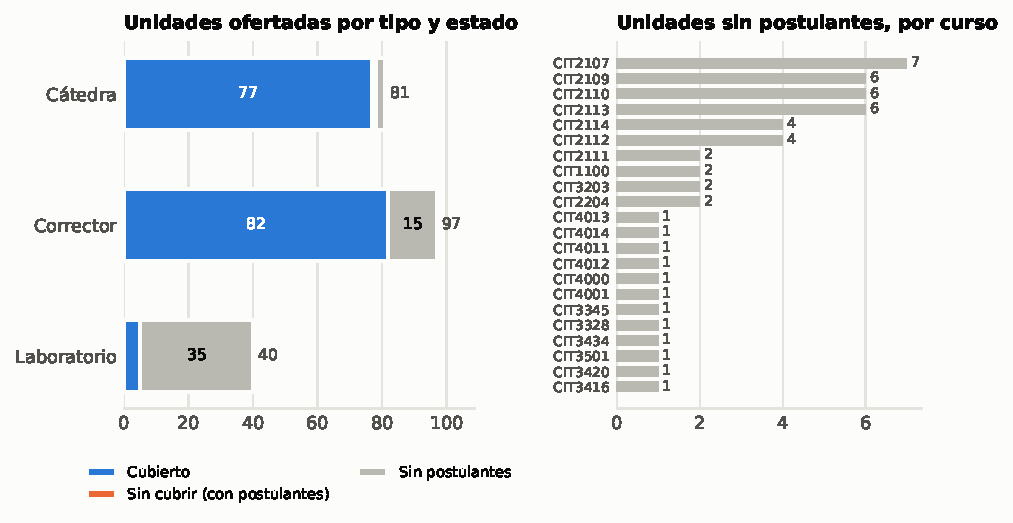
\includegraphics[width=\textwidth]{figuras/oferta.pdf}
\caption{Estado de las unidades de la oferta CIT en la solución del flujo (izquierda) y cursos con unidades sin postulantes (derecha).}
\label{fig:oferta}
\end{figure}

Este resultado marca el límite de cualquier método de asignación: \textbf{el déficit de cobertura se debe a la oferta de postulantes, no a la forma de asignar}. La falta de postulantes explica \ofSinPost{} de las \ofSinCubrir{} unidades sin cubrir. La restante, una cátedra de CIT3203, tiene un único postulante, que ya cubre el otro grupo de CIT3203 en el mismo bloque. Como el flujo es igual al flujo máximo (E6), ninguna asignación podría cubrir más unidades. Coincide con lo que señaló el Secretario: ``en esos cursos de fin de carrera hay poca demanda''.

\subsection{E3: Robustez frente al emparejamiento}
\label{sec:res-robustez}

Se resolvió el escenario base con 100 emparejamientos distintos entre secciones reconstruidas y grupos reales (Figura~\ref{fig:robustez}, Tabla~\ref{tab:robustez}). En todos ellos el flujo obtiene el 100\,\% de cobertura, cero topes y un solo no elegible; las penalizaciones de cada actor varían en unas dos centésimas. \textbf{Los indicadores principales se mantuvieron estables en los 100 emparejamientos evaluados.} Este resultado no permite establecer su sensibilidad frente a otras particiones factibles de las postulaciones, porque la partición de secciones se mantuvo fija. Tampoco mide la robustez frente a cambios reales en las postulaciones, los horarios o los cupos, que requerirían datos de otros semestres. En cambio, la asignación manual tendría entre 0 y 4 topes horarios según cuál sea el emparejamiento real.

\begin{figure}[H]
\centering
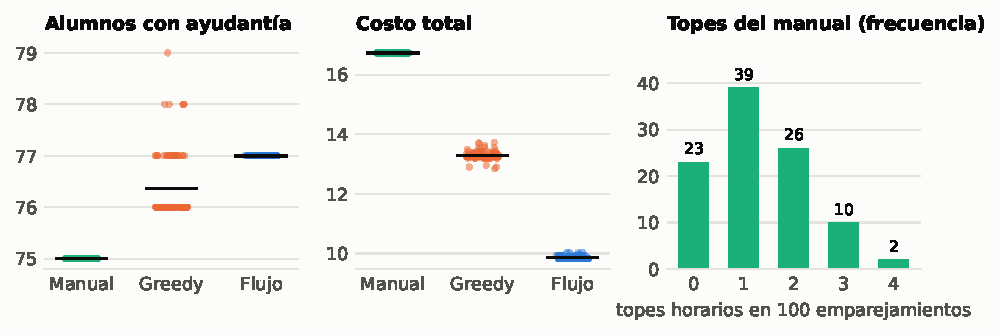
\includegraphics[width=\textwidth]{figuras/robustez.pdf}
\caption{Resultados sobre 100 emparejamientos. Cada punto es un emparejamiento; la línea negra es la media.}
\label{fig:robustez}
\end{figure}

\begin{table}[H]
\centering
\small
\begin{tabular}{lrrr}
\toprule
\textbf{Métrica} & \textbf{Manual} & \textbf{Greedy} & \textbf{Flujo} \\
\midrule
Cobertura (\%) & 100,0 & 99,2 & 100,0 \\
Alumnos con ayudantía & 75,0 & 76,4 [76,0–79,0] & 77,0 \\
Alumnos con 3 & 14,0 & 14,0 [12,0–16,0] & 15,9 [15,0–16,0] \\
Topes horarios & 1,3 [0,0–4,0] & 0,0 & 0,0 \\
No elegibles asignados & 6,0 & 4,0 [3,0–5,0] & 1,0 \\
$\bar P^O$ (profesor) & 0,113 & 0,056 [0,047–0,064] & 0,097 [0,093–0,101] \\
$\bar P^E$ (estudiante) & 0,354 & 0,331 [0,323–0,342] & 0,246 [0,240–0,261] \\
$\bar P^A$ (asignatura) & 0,356 & 0,314 [0,302–0,326] & 0,231 [0,225–0,242] \\
Costo total & 16,73 & 13,29 [12,85–13,73] & 9,86 [9,83–10,04] \\
\bottomrule
\end{tabular}

\caption{Media [mínimo--máximo] sobre 100 emparejamientos (sin intervalo cuando el valor es constante).}
\label{tab:robustez}
\end{table}

\subsection{E4: Selección de los pesos $a$, $b$, $c$}
\label{sec:res-pesos}

Se resolvió el escenario base para las \pesosN{} proporciones $a : b : c$ del triángulo con paso 0,1 (manteniendo $d = \pesoD$ y reescalando para que $a + b + c + d = 1$), promediando cada una sobre \pesosSemillas{} emparejamientos. La cobertura es 100\,\% en todas, porque el criterio lexicográfico la protege; lo que cambia es quién obtiene su primera opción (Figura~\ref{fig:pesos}). Cada vértice favorece a un actor a costa de los otros dos: en el vértice del profesor (proporción $1 : 0 : 0$; pesos efectivos $a = 0{,}4$, $b = c = 0$), $\bar P^O$ es mínimo pero $\bar P^E$ y $\bar P^A$ son altos.

\begin{figure}[H]
\centering
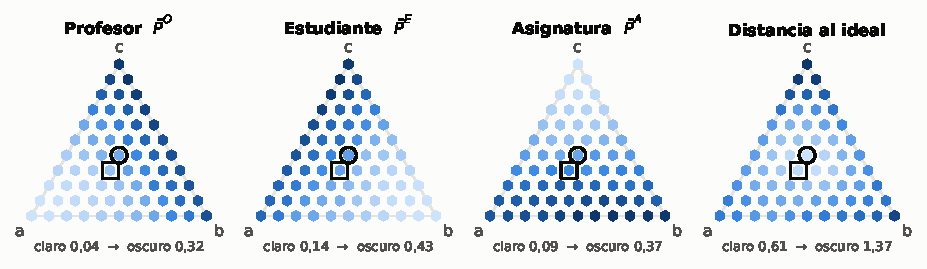
\includegraphics[width=\textwidth]{figuras/pesos.pdf}
\caption{Penalización media de cada actor y distancia al ideal sobre el triángulo de pesos (vértices: $a$ profesor, $b$ estudiante, $c$ asignatura). Más claro es mejor. $\circ$: compromiso libre; $\square$: compromiso con la jerarquía del Secretario.}
\label{fig:pesos}
\end{figure}

Para elegir un punto se aplicó programación de compromiso~\cite{zeleny1982}: cada $\bar P$ se normaliza entre su mejor y su peor valor en el triángulo y se mide la distancia euclidiana al punto ideal $(0, 0, 0)$:
\[
    \tilde P^k = \frac{\bar P^k - \text{ideal}_k}{\text{anti-ideal}_k - \text{ideal}_k}, \qquad
    D = \sqrt{(\tilde P^O)^2 + (\tilde P^E)^2 + (\tilde P^A)^2}, \qquad k \in \{O, E, A\}.
\]
El ideal y el anti-ideal de cada actor son el mínimo y el máximo observados de su penalización media sobre las \pesosN{} proporciones (Tabla~\ref{tab:ideal-nadir}). El anti-ideal no coincide con ningún vértice del triángulo, por lo que no puede leerse en la Tabla~\ref{tab:pesos}.

% cifras transcritas a mano desde salidas/resultados.xlsx, hoja "E4 pesos (triángulo)"
\begin{table}[H]
\centering
\small
\begin{tabular}{lrr}
\toprule
\textbf{Actor} & \textbf{Ideal} & \textbf{Anti-ideal} \\
\midrule
Profesor ($\bar P^O$) & 0,045 & 0,321 \\
Estudiante ($\bar P^E$) & 0,143 & 0,431 \\
Asignatura ($\bar P^A$) & 0,087 & 0,370 \\
\bottomrule
\end{tabular}
\caption{Ideal y anti-ideal de cada actor en el triángulo de pesos (media sobre \pesosSemillas{} emparejamientos).}
\label{tab:ideal-nadir}
\end{table}

La condición de jerarquía no cambia la normalización: solo restringe la búsqueda del mínimo de $D$ a los puntos con $a \geq b$ y $a \geq c$. Se reportan dos óptimos:
\begin{itemize}
    \item \textbf{Compromiso libre} (proporción $a : b : c = \libreA : \libreB : \libreC$): minimiza la distancia normalizada al ideal sin imponer una jerarquía entre los actores.
    \item \textbf{Compromiso con jerarquía} (proporción $a : b : c = \jerA : \jerB : \jerC$): el más cercano al ideal entre los puntos con $a \geq b$ y $a \geq c$, que respetan el criterio del Secretario de que ``la prioridad del alumno pasa a segundo plano'' frente a la del profesor. Respecto del libre, sube la primera preferencia del profesor de \librePrimProf\,\% a \jerPrimProf\,\% y la proporción dentro de sus tres primeros de \libreTresProf\,\% a \jerTresProf\,\%.
\end{itemize}
Se adoptó el \textbf{compromiso con jerarquía} como proporción por defecto; con $d = \pesoD$ los pesos efectivos son $a/b/c = \pesoA/\pesoB/\pesoC$. La Tabla~\ref{tab:pesos} sirve al Secretario como menú: muestra cuánto gana cada actor y cuánto cede en cada extremo.

\begin{table}[H]
\centering
\small
\resizebox{\textwidth}{!}{\begin{tabular}{lrrrrrrrrrr}
\toprule
\textbf{Configuración} & \textbf{a} & \textbf{b} & \textbf{c} & \textbf{$\bar P^O$} & \textbf{$\bar P^E$} & \textbf{$\bar P^A$} & \textbf{1ª prof. (\%)} & \textbf{Top 3 prof. (\%)} & \textbf{Alumnos} & \textbf{Dist.} \\
\midrule
Solo profesor & 1,0 & 0,0 & 0,0 & 0,045 & 0,338 & 0,309 & 85,7 & 100,0 & 77,1 & 1,036 \\
Solo estudiante & 0,0 & 1,0 & 0,0 & 0,273 & 0,143 & 0,365 & 43,5 & 76,9 & 85,0 & 1,281 \\
Solo asignatura & 0,0 & 0,0 & 1,0 & 0,311 & 0,422 & 0,087 & 34,0 & 76,3 & 63,3 & 1,366 \\
Compromiso libre ($\circ$) & 0,3 & 0,3 & 0,4 & 0,134 & 0,253 & 0,185 & 56,3 & 92,8 & 74,7 & 0,609 \\
Con jerarquía ($\square$) & 0,4 & 0,3 & 0,3 & 0,097 & 0,245 & 0,230 & 63,0 & 96,7 & 77,0 & 0,648 \\
\bottomrule
\end{tabular}
}
\caption{Configuraciones de referencia (proporciones $a : b : c$; media sobre \pesosSemillas{} emparejamientos). ``Top 3 prof.'': asignaciones dentro de los tres primeros del profesor.}
\label{tab:pesos}
\end{table}

\subsection{E5: Postulantes no elegibles y elección de $d$}
\label{sec:res-elegibilidad}

Se probaron cinco umbrales de elegibilidad (promedio mínimo / nota mínima del ramo) y once modos: excluir, dos pasadas, penalizar con $d \in \{0{,}05; 0{,}1; 0{,}2; 0{,}3; 0{,}4; 0{,}5; 0{,}6; 0{,}8\}$ (manteniendo la proporción $a : b : c$ y reescalando para que la suma siga siendo 1) y sin criterio ($d = 0$).

\begin{figure}[H]
\centering
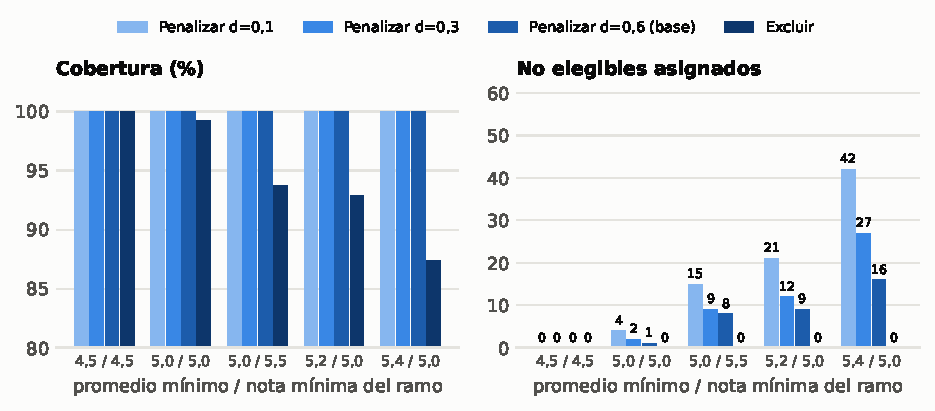
\includegraphics[width=\textwidth]{figuras/no_elegibles.pdf}
\caption{Cobertura y no elegibles asignados por umbral y modo (de más flexible, claro, a más estricto, oscuro).}
\label{fig:no-elegibles}
\end{figure}

\begin{table}[H]
\centering
\small
\begin{tabular}{lrrrrrrr}
\toprule
\textbf{Modo} & \textbf{Cubiertos} & \textbf{No eleg.} & \textbf{Alumnos} & \textbf{1ª prof. (\%)} & \textbf{$\bar P^O$} & \textbf{$\bar P^E$} & \textbf{$\bar P^A$} \\
\midrule
Excluir & 126 & 0 & 76 & 62,7 & 0,101 & 0,241 & 0,227 \\
Dos pasadas & 127 & 1 & 77 & 63,0 & 0,100 & 0,239 & 0,233 \\
Penalizar d = 0,05 & 127 & 5 & 80 & 65,4 & 0,075 & 0,238 & 0,233 \\
Penalizar d = 0,1 & 127 & 4 & 79 & 66,1 & 0,075 & 0,242 & 0,231 \\
Penalizar d = 0,2 & 127 & 3 & 78 & 64,6 & 0,085 & 0,247 & 0,218 \\
Penalizar d = 0,3 & 127 & 2 & 77 & 63,0 & 0,092 & 0,248 & 0,217 \\
Penalizar d = 0,4 & 127 & 2 & 77 & 63,0 & 0,092 & 0,248 & 0,217 \\
Penalizar d = 0,5 & 127 & 1 & 77 & 63,0 & 0,097 & 0,245 & 0,230 \\
Penalizar d = 0,6 & 127 & 1 & 77 & 63,0 & 0,097 & 0,245 & 0,230 \\
Penalizar d = 0,8 & 127 & 1 & 76 & 63,0 & 0,095 & 0,251 & 0,228 \\
Sin criterio (d = 0) & 127 & 7 & 82 & 66,1 & 0,080 & 0,227 & 0,234 \\
\bottomrule
\end{tabular}

\caption{Todos los modos con el umbral base (\elegPromMin{} / \elegNotaMin).}
\label{tab:no-elegibles}
\end{table}

\begin{table}[H]
\centering
\small
\resizebox{\textwidth}{!}{\begin{tabular}{lrrrrrr}
\toprule
\textbf{Umbral} & \textbf{Post. no eleg.} & \textbf{Excluir: cub.} & \textbf{2 pasadas: cub.} & \textbf{2 pasadas: no eleg.} & \textbf{$d=0{,}6$: cub.} & \textbf{$d=0{,}6$: no eleg.} \\
\midrule
4,5 / 4,5 & 57 & 127 & 127 & 0 & 127 & 0 \\
5,0 / 5,0 & 251 & 126 & 127 & 1 & 127 & 1 \\
5,0 / 5,5 & 462 & 119 & 127 & 8 & 127 & 8 \\
5,2 / 5,0 & 398 & 118 & 127 & 9 & 127 & 9 \\
5,4 / 5,0 & 681 & 111 & 127 & 16 & 127 & 16 \\
\bottomrule
\end{tabular}
}
\caption{Efecto del umbral: unidades cubiertas al excluir, y no elegibles que usan las dos pasadas y el peso $d = 0{,}6$.}
\label{tab:umbrales}
\end{table}

Los resultados muestran tres comportamientos:
\begin{itemize}
    \item \textbf{Excluir} nunca usa no elegibles, pero pierde cobertura en cuanto el umbral es exigente (\neExcluirCub{} de 127 con el umbral base). Es lo que el Secretario resolvería después a mano, con la hoja \emph{Decisión manual}.
    \item \textbf{Dos pasadas} mantiene el 100\,\% en todos los umbrales usando el \textbf{mínimo de no elegibles necesarios} (\neDosNo{} con el umbral base): la primera pasada es el máximo flujo posible solo con elegibles, así que ninguna asignación completa puede usar menos.
    \item \textbf{Penalizar} recorre todo el rango entre ambos extremos según $d$: con $d = 0{,}05$ entran \nePenChicoNo{} no elegibles, con $d = 0{,}3$ entran \nePenMedioNo{} y sin criterio \neSinCritNo; con $d = 0{,}6$, \nePenGrandeNo, el mínimo.
\end{itemize}

\paragraph{Elección de $d$.} Para fijar el valor por defecto se midió, para cada $d$ y cada umbral, cuántos no elegibles usa el flujo \emph{por sobre el mínimo necesario}, tomando el peor caso entre 5 emparejamientos (Tabla~\ref{tab:exceso-d}). En ningún caso se perdió cobertura respecto de las dos pasadas.

\begin{table}[H]
\centering
\small
\begin{tabular}{rrrrrr}
\toprule
\textbf{d} & \textbf{4,5 / 4,5} & \textbf{5,0 / 5,0} & \textbf{5,0 / 5,5} & \textbf{5,2 / 5,0} & \textbf{5,4 / 5,0} \\
\midrule
0,05 & 0 & 5 & 12 & 15 & 29 \\
0,10 & 0 & 4 & 8 & 13 & 26 \\
0,20 & 0 & 2 & 3 & 8 & 20 \\
0,30 & 0 & 1 & 1 & 4 & 12 \\
0,40 & 0 & 1 & 0 & 2 & 5 \\
0,50 & 0 & 0 & 0 & 1 & 0 \\
0,60 & 0 & 0 & 0 & 0 & 0 \\
0,80 & 0 & 0 & 0 & 0 & 0 \\
\bottomrule
\end{tabular}

\caption{No elegibles asignados por sobre el mínimo necesario, peor caso en 5 emparejamientos, por valor de $d$ (filas) y umbral promedio / nota (columnas). 0 significa que no se usaron no elegibles adicionales a los necesarios para alcanzar la cobertura obtenida, considerando conjuntamente todas las restricciones.}
\label{tab:exceso-d}
\end{table}

Desde $d = \neDCritico$ el exceso es cero en todos los umbrales y emparejamientos evaluados: en esos casos no se usaron no elegibles adicionales a los necesarios para alcanzar la cobertura obtenida, considerando conjuntamente todas las restricciones de asignación. Esto no significa que cada unidad asignada a un no elegible careciera de candidatos elegibles: estos pueden ser necesarios en otras unidades. Es un resultado empírico; la garantía formal de usar el mínimo la da el modo de dos pasadas (Sección~\ref{sec:algoritmo}). Se adoptó $d = \pesoD$, el \textbf{menor} valor con esa propiedad, porque deja el mayor peso posible a las tres preferencias. Reproduce la regla del Secretario (``tengo tres no elegibles, [...] pa' adentro un no elegible'', pero ``si me hubiera postulado un elegible, tengo que hablar de elegible'') y, si quiere más flexibilidad, basta con bajar $d$ en \texttt{parametros.json}; la tabla muestra cuántos no elegibles adicionales implicaría cada valor. Los modos dos pasadas y excluir quedan disponibles como alternativas estrictas.

El umbral base de \elegPromMin{} es el más exigente de los probados que mantiene la cobertura con a lo más un no elegible; con 5,2 o 5,4 de promedio hacen falta 9 y 16.

\subsection{E6: Verificación del criterio lexicográfico}

\begin{table}[H]
\centering
\small
\begin{tabular}{lrrrrrrr}
\toprule
\textbf{Escenario} & \textbf{Cupos} & \textbf{Nodos} & \textbf{Aristas} & \textbf{Flujo máx.} & \textbf{Flujo SSP} & \textbf{Tiempo (ms)} & \textbf{Dos pasadas} \\
\midrule
histórico & 127 & 723 & 1.677 & 127 & 127 & 74 & 127 \\
todas & 160 & 771 & 1.989 & 159 & 159 & 107 & 159 \\
oferta & 218 & 785 & 2.028 & 164 & 164 & 121 & 164 \\
\bottomrule
\end{tabular}

\caption{Flujo del SSP (todas las aristas) comparado con el flujo máximo sin costos, calculado con \texttt{networkx}, y flujo total de las dos pasadas.}
\label{tab:lexico}
\end{table}

En los tres escenarios de cupos, el flujo del SSP coincide con el flujo máximo calculado sin costos (Tabla~\ref{tab:lexico}): las preferencias nunca sacrifican cobertura. Las dos pasadas alcanzan el mismo flujo total, es decir, en estos datos priorizar a los elegibles tampoco cuesta cobertura. En el escenario ``todas'' (160 cupos), ni el flujo máximo alcanza 160: los dos grupos de CIT3203 tienen ayudantía el miércoles a las 16:00 y un mismo alumno es el único postulante de ambos.

\subsection{E7: Capacidades}
\label{sec:res-capacidades}

\begin{table}[H]
\centering
\small
\resizebox{\textwidth}{!}{\begin{tabular}{lrrrrrr}
\toprule
\textbf{Variante} & \textbf{Cubiertos (127)} & \textbf{Alumnos (127)} & \textbf{Con 3} & \textbf{1ª prof. (\%)} & \textbf{Cubiertos (218)} & \textbf{Alumnos (218)} \\
\midrule
Máx. 1 por alumno & 125 & 125 & 0 & 47,2 & 147 & 147 \\
Máx. 2 por alumno & 127 & 82 & 0 & 59,1 & 164 & 101 \\
Máx. 3 por alumno (base) & 127 & 77 & 16 & 63,0 & 164 & 91 \\
Máx. 4 por alumno & 127 & 75 & 15 & 61,4 & 164 & 88 \\
Corrección cap. 1 & 127 & 84 & 11 & 58,3 & 163 & 105 \\
Corrección cap. 2 & 127 & 78 & 13 & 60,6 & 164 & 93 \\
Sin no rankeados & 127 & 77 & 16 & 63,0 & 159 & 89 \\
\bottomrule
\end{tabular}
}
\caption{Efecto del tope por alumno, de la capacidad del bloque de corrección y de incluir a los no rankeados, en el escenario histórico (127 cupos) y en toda la oferta.}
\label{tab:capacidades}
\end{table}

\begin{itemize}
    \item \textbf{Tope por alumno.} Con 1 solo se cubren \capUnoCub{} de 127. Con 2 se cubren \capDosCub{} y se reparte entre \capDosAlumnos{} alumnos, sin nadie con 3, a cambio de bajar la primera preferencia del profesor a \capDosPrim\,\%. Con 4 el resultado prácticamente no cambia respecto de 3. Es decir, en el escenario histórico existe una asignación factible con cobertura completa y nadie con más de 2, cercana al ideal del Secretario (``ojalá que todos tengan 2''). Se obtiene con una capacidad, sin costos adicionales, aunque el modelo no optimiza la equidad de forma explícita.
    \item \textbf{Bloque de corrección.} Con capacidad 1 en vez de 3, en toda la oferta se cubren \capCorrUnoOf{} unidades en lugar de \capBaseOf: limitar la corrección a una por alumno no tiene fundamento, porque no ocupa horario.
    \item \textbf{No rankeados.} Excluirlos no cambia el escenario histórico, pero en toda la oferta baja la cobertura de \capBaseOf{} a \capSinRankOf: el orden por defecto rescata unidades cuyos profesores no rankearon.
\end{itemize}

% =====================================================================
\section{Discusión}

\paragraph{Qué aporta el modelo.} Con la misma cobertura que el proceso manual, el flujo elimina los topes horarios, usa solo los no elegibles imprescindibles y deja listados los casos dudosos para el Secretario, y mejora la posición que obtienen los alumnos y el mérito de los asignados. Hoy el Secretario logra una cobertura equivalente con un día de ajustes manuales; el modelo lo hace en una fracción de segundo, de forma reproducible y con los criterios escritos en un archivo, lo que responde a la demanda de transparencia de la encuesta.

\paragraph{Qué se cede.} Respecto de una selección local por curso, el flujo da menos veces la primera preferencia del profesor. Es una consecuencia de optimizar el sistema completo y de dar peso también al alumno y al mérito: el profesor no sabe que su primer candidato postuló a muchos cursos (``todos también lo querían a él''). Los pesos $a$, $b$, $c$ permiten mover este equilibrio de manera explícita (Tabla~\ref{tab:pesos}).

\paragraph{Simplicidad frente a expresividad.} El modelo tiene una sola arista con costo, y todas las reglas institucionales son capacidades o parte de la estructura. Esto lo hace más fácil de explicar (``nadie puede tener más de 3'', ``un no elegible entra solo si hace falta para cubrir'', garantizado en dos pasadas y observado con $d = \pesoD$) y más fácil de auditar. El reparto de ayudantías, que podría haberse incentivado con costos, se controla directamente con la capacidad (E7).

\paragraph{Limitaciones.}
\begin{itemize}
    \item El emparejamiento entre secciones reconstruidas y grupos reales es un supuesto. En los 100 emparejamientos evaluados en E3, los indicadores principales se mantuvieron estables; esto no demuestra robustez frente a otras particiones posibles ni frente a datos de otros semestres.
    \item No se consideran los topes con los ramos propios del alumno (supuesto 3).
    \item La elegibilidad se calcula con umbrales de notas; el dato oficial puede cargarse a mano en la plantilla.
    \item Los pesos recomendados son sintéticos: resultan de un criterio de compromiso, no de una calibración con el Secretario.
    \item Se supone un ayudante por grupo y tipo.
    \item La reconstrucción de secciones es una partición factible, no necesariamente la original, y las 5 secciones sin par en la oferta no tienen control de topes.
\end{itemize}

% =====================================================================
\section{Conclusiones y trabajo futuro}

Se implementó y evaluó el modelo de flujo máximo de costo mínimo propuesto en la Entrega 1, con datos reales del semestre. La Tabla~\ref{tab:cumplimiento} contrasta la situación actual con el resultado obtenido para cada objetivo, y distingue lo que es una \emph{garantía} del método (vale para cualquier dato) de lo que es un resultado \emph{empírico} de los datos de 2026-2.

\begin{table}[H]
\centering
\small
\begin{tabularx}{\textwidth}{l >{\raggedright\arraybackslash}X >{\raggedright\arraybackslash}X >{\raggedright\arraybackslash}X >{\raggedright\arraybackslash}p{2.6cm}}
\toprule
\textbf{Obj.} & \textbf{Indicador} & \textbf{Situación actual} & \textbf{Modelo (escenario base)} & \textbf{Respaldo} \\
\midrule
Principal & Tiempo y forma de obtener la asignación & $\sim$1 día de ajustes manuales & $\sim$0,1 s, reproducible, con parámetros registrados & Empírico \\
OE1 & Violaciones de restricciones duras & 0 excesos del tope, 3 topes horarios entre ayudantías & 0 en todos los escenarios y emparejamientos (E1, E3), entre ayudantías con bloque conocido; las unidades sin bloque conocido requieren validación manual (por ejemplo, los dos laboratorios de CIT2108 asignados a P026) & Garantía (capacidades), condicionada a los bloques conocidos \\
OE2 & Peso explícito de cada actor & implícito & $a/b/c = \pesoA/\pesoB/\pesoC$, elegidos con E4 & Empírico (E4) \\
OE3 & Cobertura (127 unidades) & 100\,\% & 100\,\%, igual al flujo máximo (E6) & Garantía (T2, T3) \\
OE4 & No elegibles asignados & \hNoEleg, decididos a mano & \fNoEleg, el mínimo necesario, y listados (E5) & Garantía en dos pasadas; empírico con $d$ \\
OE5 & Métricas y comparación & no existían & 3 métodos, 7 experimentos & Empírico \\
\bottomrule
\end{tabularx}
\caption{Cumplimiento de los objetivos.}
\label{tab:cumplimiento}
\end{table}

Como continuación se proponen:

\begin{enumerate}
    \item \textbf{Calibración de los pesos con el Secretario Académico}, usando la Tabla~\ref{tab:pesos} como menú y, si es posible, sus decisiones de semestres anteriores para estimar los pesos que mejor las reproducen.
    \item \textbf{Integración con la plataforma de postulación y SAP}, para usar el dato oficial de elegibilidad y las ayudantías de Ciencias Básicas en lugar de cargarlos a mano.
    \item \textbf{Modelo en dos etapas ante imprevistos.} La primera etapa es la asignación actual; la segunda, un flujo de reemplazo de costo mínimo sobre la red residual ante renuncias o topes descubiertos después (por ejemplo, con ramos propios, que hoy se suponen inexistentes).
    \item \textbf{Variables de malla y salud mental} (avance, ramos atrasados, horas libres), que entrarían como reducción individual de la capacidad $k_i$, coherente con la regla de modelar lo duro como capacidad.
    \item \textbf{Fomento de la postulación} en las unidades sin postulantes que identifica E2.
\end{enumerate}

% =====================================================================
\begin{thebibliography}{99}

\bibitem{palma2025uta}
C. D. Palma, P. González-Brevis, P. A. Riffo y N. S. Montenegro,
``A Proposed Mathematical Optimization Approach for Undergraduate
Teaching Assistant Selection and Tutorial Scheduling,''
\textit{INFORMS Transactions on Education},
vol. 26, no. 3, pp. 175--186, 2025.
doi: 10.1287/ited.2024.0095.

\bibitem{abraham2007spa}
D. J. Abraham, R. W. Irving y D. F. Manlove,
``Two Algorithms for the Student-Project Allocation Problem,''
\textit{Journal of Discrete Algorithms},
vol. 5, no. 1, pp. 73--90, 2007.
doi: 10.1016/j.jda.2006.03.006.

\bibitem{qu2017ta}
X. Qu, W. Yi, T. Wang, S. Wang, L. Xiao y Z. Liu,
``Mixed-Integer Linear Programming Models for Teaching Assistant
Assignment and Extensions,''
\textit{Scientific Programming},
vol. 2017, Article ID 9057947, 2017.
doi: 10.1155/2017/9057947.

\bibitem{guler2015ta}
M. G. Güler, M. E. Keskin, A. Döyen y H. Akyer,
``On Teaching Assistant-Task Assignment Problem: A Case Study,''
\textit{Computers \& Industrial Engineering},
vol. 79, pp. 18--26, 2015.
doi: 10.1016/j.cie.2014.10.004.

\bibitem{ahuja1993}
R. K. Ahuja, T. L. Magnanti y J. B. Orlin,
\textit{Network Flows: Theory, Algorithms, and Applications}.
Prentice Hall, 1993.

\bibitem{edmonds1972}
J. Edmonds y R. M. Karp,
``Theoretical Improvements in Algorithmic Efficiency for Network Flow Problems,''
\textit{Journal of the ACM},
vol. 19, no. 2, pp. 248--264, 1972.
doi: 10.1145/321694.321699.

\bibitem{kuhn1955}
H. W. Kuhn,
``The Hungarian Method for the Assignment Problem,''
\textit{Naval Research Logistics Quarterly},
vol. 2, no. 1--2, pp. 83--97, 1955.

\bibitem{klein1967}
M. Klein,
``A Primal Method for Minimal Cost Flows with Applications to the Assignment and Transportation Problems,''
\textit{Management Science},
vol. 14, no. 3, pp. 205--220, 1967.

\bibitem{goldberg1990}
A. V. Goldberg y R. E. Tarjan,
``Finding Minimum-Cost Circulations by Successive Approximation,''
\textit{Mathematics of Operations Research},
vol. 15, no. 3, pp. 430--466, 1990.

\bibitem{orlin1997}
J. B. Orlin,
``A Polynomial Time Primal Network Simplex Algorithm for Minimum Cost Flows,''
\textit{Mathematical Programming},
vol. 78, no. 2, pp. 109--129, 1997.

\bibitem{tomizawa1971}
N. Tomizawa,
``On Some Techniques Useful for Solution of Transportation Network Problems,''
\textit{Networks},
vol. 1, no. 2, pp. 173--194, 1971.

\bibitem{fordfulkerson1956}
L. R. Ford y D. R. Fulkerson,
``Maximal Flow through a Network,''
\textit{Canadian Journal of Mathematics},
vol. 8, pp. 399--404, 1956.

\bibitem{busacker1960}
R. G. Busacker y P. J. Gowen,
``A Procedure for Determining a Family of Minimum-Cost Network Flow Patterns,''
ORO Technical Paper 15, Operations Research Office, Johns Hopkins University, 1960.

\bibitem{zeleny1982}
M. Zeleny,
\textit{Multiple Criteria Decision Making}.
McGraw-Hill, 1982.

\end{thebibliography}

% =====================================================================
\appendix
\section{Parámetros (\texttt{parametros.json})}
\label{sec:anexo-param}

\begin{table}[H]
\centering
\small
\begin{tabularx}{\textwidth}{l l >{\raggedright\arraybackslash}X}
\toprule
\textbf{Parámetro} & \textbf{Valor base} & \textbf{Origen} \\
\midrule
$a$ (profesor), $b$ (estudiante), $c$ (asignatura) & \pesoA{} / \pesoB{} / \pesoC & Sintético: proporción \propA{} : \propB{} : \propC{} del compromiso con jerarquía (E4), reescalada a $1 - d$; en la práctica los fija el Secretario \\
$d$ (no elegible) & \pesoD & Menor valor que no usa más no elegibles que los necesarios para la cobertura (E5) \\
\texttt{max\_ayudantias} & 3 & Norma del Secretario; E7 \\
\texttt{capacidad\_correccion} & 3 & La corrección no ocupa bloque; E7 \\
\texttt{cupos} & \texttt{historico} & Unidades con ayudante en 2026-2 \\
\texttt{incluir\_no\_rankeados} & sí & Orden por defecto; E7 \\
\texttt{promedio\_minimo}, \texttt{nota\_minima\_ramo} & \elegPromMin{} / \elegNotaMin & Entrada del usuario; E5 \\
\texttt{modo\_no\_elegibles} & \texttt{penalizar} & Usa $d$; \texttt{excluir} no los toma en cuenta; \texttt{dos\_pasadas} (E5) \\
\texttt{archivo\_elegibilidad} & ninguno & Plantilla exportada por \texttt{main.py} \\
\texttt{externas} & vacío & Ayudantías en otros departamentos (entrada del usuario) \\
\texttt{semilla} & 0 & Emparejamiento sección--grupo (E3) \\
\bottomrule
\end{tabularx}
\caption{Parámetros por defecto. Todos se editan a mano en \texttt{parametros.json}; el programa valida que $a + b + c + d = 1$.}
\end{table}

\section{Reproducibilidad}

\begin{verbatim}
python3 -m venv .venv && .venv/bin/pip install -r requirements.txt
.venv/bin/python main.py                          # asignación -> salidas/asignacion.xlsx
.venv/bin/python main.py --exportar-elegibilidad  # plantilla de elegibilidad
.venv/bin/python main.py --cupos oferta           # toda la oferta
.venv/bin/python experimentos.py                  # E1-E7 -> salidas/resultados.xlsx
.venv/bin/python informe/generar_figuras.py       # figuras, tablas y cifras
.venv/bin/python -m pytest tests                  # 31 pruebas
\end{verbatim}

\section{Asignación propuesta}

La Tabla~\ref{tab:anexo} lista la asignación completa del escenario base, con identificadores anónimos. ``R. prof.'' es la posición en el ranking del profesor (con * si se completó con el orden por defecto), ``P. alum.'' la prioridad del alumno y ``Eleg.'' si cumple el criterio de elegibilidad.

{\small
\begin{longtable}{llllrrcl}
\caption{Asignación completa propuesta por el flujo (escenario base).}\label{tab:anexo}\\
\toprule
\textbf{Sigla} & \textbf{Tipo} & \textbf{Unidad} & \textbf{Alumno} & \textbf{R. prof.} & \textbf{P. alum.} & \textbf{Eleg.} & \textbf{Bloque} \\
\midrule
\endfirsthead
\toprule
\textbf{Sigla} & \textbf{Tipo} & \textbf{Unidad} & \textbf{Alumno} & \textbf{R. prof.} & \textbf{P. alum.} & \textbf{Eleg.} & \textbf{Bloque} \\
\midrule
\endhead
\bottomrule
\endfoot
CIT1100 & Corrector & CIT1100-COR-G03 & P059 & 2 & 6 & sí & — \\
CIT1100 & Corrector & CIT1100-COR-G02 & P121 & 1 & 1 & sí & — \\
CIT1100 & Corrector & CIT1100-COR-G01 & P059 & 2 & 4 & sí & — \\
CIT1100 & Corrector & CIT1100-COR-G06 & P086 & 1 & 5 & sí & — \\
CIT1100 & Cátedra & CIT1100-CAT-G05 & P086 & 1 & 1 & sí & MI 17:25 \\
CIT1100 & Cátedra & CIT1100-CAT-G02 & P066 & 5 & 1 & sí & MI 11:30 \\
CIT1100 & Cátedra & CIT1100-CAT-G06 & P086 & 8 & 6 & sí & MI 08:30 \\
CIT1100 & Cátedra & CIT1100-CAT-G03 & P136 & 3 & 4 & sí & LU 13:00 \\
CIT1110 & Corrector & CIT1110-COR-G07 & P125 & 2 & 2 & sí & — \\
CIT1110 & Corrector & CIT1110-COR-G04 & P064 & 3 & 3 & sí & — \\
CIT1110 & Corrector & CIT1110-COR-G01 & P080 & 2 & 17 & sí & — \\
CIT1110 & Corrector & CIT1110-COR-G06 & P075 & 1 & 1 & sí & — \\
CIT1110 & Corrector & CIT1110-COR-G03 & P099 & 3 & 9 & sí & — \\
CIT1110 & Corrector & CIT1110-COR-G02 & P147 & 2 & 1 & sí & — \\
CIT1110 & Corrector & CIT1110-COR-G05 & P062 & 3 & 3 & sí & — \\
CIT1110 & Cátedra & CIT1110-CAT-G03 & P062 & 5 & 1 & sí & MA 11:30 \\
CIT1110 & Cátedra & CIT1110-CAT-G01 & P081 & 1 & 1 & sí & JU 13:00 \\
CIT1110 & Cátedra & CIT1110-CAT-G04 & P105 & 1 & 6 & sí & MA 16:00 \\
CIT1110 & Cátedra & CIT1110-CAT-G02 & P100 & 2 & 1 & sí & JU 10:00 \\
CIT1110 & Cátedra & CIT1110-CAT-G07 & P135 & 2 & 10 & sí & MA 17:25 \\
CIT1110 & Cátedra & CIT1110-CAT-G06 & P135 & 1 & 8 & sí & JU 14:30 \\
CIT1110 & Cátedra & CIT1110-CAT-G05 & P099 & 1 & 1 & sí & MI 10:00 \\
CIT2006 & Cátedra & CIT2006-CAT-G01 & P014 & 1 & 7 & sí & MI 11:30 \\
CIT2006 & Cátedra & CIT2006-CAT-G02 & P105 & 1 & 4 & sí & MI 08:30 \\
CIT2006 & Cátedra & CIT2006-CAT-G03 & P014 & 3 & 1 & sí & VI 11:30 \\
CIT2006 & Laboratorio & CIT2006-LAB-03 & P074 & 1 & 2 & sí & LU 11:30 \\
CIT2006 & Laboratorio & CIT2006-LAB-01 & P014 & 2 & 3 & sí & MA 13:00 \\
CIT2006 & Laboratorio & CIT2006-LAB-02 & P074 & 1 & 1 & sí & JU 08:30 \\
CIT2007 & Corrector & CIT2007-COR-G05 & P012 & 2 & 4 & sí & — \\
CIT2007 & Corrector & CIT2007-COR-G01 & P059 & 3 & 1 & sí & — \\
CIT2007 & Corrector & CIT2007-COR-G02 & P125 & 1 & 4 & sí & — \\
CIT2007 & Corrector & CIT2007-COR-G03 & P040 & 1 & 2 & sí & — \\
CIT2007 & Cátedra & CIT2007-CAT-G01 & P016 & 1 & 1 & sí & LU 08:30 \\
CIT2007 & Cátedra & CIT2007-CAT-G03 & P110 & 1 & 1 & sí & LU 08:30 \\
CIT2007 & Cátedra & CIT2007-CAT-G02 & P127 & 1 & 1 & sí & MI 10:00 \\
CIT2007 & Cátedra & CIT2007-CAT-G04 & P074 & 1 & 3 & sí & VI 13:00 \\
CIT2007 & Cátedra & CIT2007-CAT-G05 & P149 & 1 & 2 & sí & VI 13:00 \\
CIT2008 & Cátedra & CIT2008-CAT-G03 & P016 & 1 & 19 & sí & MI 16:00 \\
CIT2008 & Cátedra & CIT2008-CAT-G05 & P022 & 1 & 6 & sí & MI 11:30 \\
CIT2008 & Cátedra & CIT2008-CAT-G02 & P078 & 1 & 4 & sí & LU 11:30 \\
CIT2008 & Cátedra & CIT2008-CAT-G04 & P016 & 3 & 9 & sí & MA 13:00 \\
CIT2008 & Cátedra & CIT2008-CAT-G01 & P055 & 1 & 1 & sí & MI 14:30 \\
CIT2009 & Corrector & CIT2009-COR-G01 & P085 & 2 & 2 & sí & — \\
CIT2009 & Cátedra & CIT2009-CAT-G02 & P111 & 1 & 1 & sí & MA 17:25 \\
CIT2009 & Cátedra & CIT2009-CAT-G01 & P011 & 1 & 1 & sí & MI 16:00 \\
CIT2010 & Corrector & CIT2010-COR-G01 & P015 & 2 & 1 & sí & — \\
CIT2010 & Corrector & CIT2010-COR-G03 & P041 & 1 & 1 & sí & — \\
CIT2010 & Corrector & CIT2010-COR-G02 & P044 & 1 & 10 & sí & — \\
CIT2010 & Cátedra & CIT2010-CAT-G03 & P133 & 1 & 1 & sí & MI 14:30 \\
CIT2010 & Cátedra & CIT2010-CAT-G04 & P135 & 1 & 2 & sí & VI 13:00 \\
CIT2010 & Cátedra & CIT2010-CAT-G01 & P093 & 1 & 1 & sí & MI 17:25 \\
CIT2010 & Cátedra & CIT2010-CAT-G02 & P113 & 2 & 5 & sí & MI 17:25 \\
CIT2011 & Corrector & CIT2011-COR-G02 & P102 & 2 & 2 & sí & — \\
CIT2011 & Corrector & CIT2011-COR-G01 & P102 & 1 & 1 & sí & — \\
CIT2011 & Cátedra & CIT2011-CAT-G02 & P032 & 1 & 1 & sí & MI 17:25 \\
CIT2011 & Cátedra & CIT2011-CAT-G01 & P117 & 2 & 2 & sí & MI 17:25 \\
CIT2012 & Cátedra & CIT2012-CAT-G01 & P139 & 2 & 1 & sí & MI 16:00 \\
CIT2013 & Corrector & CIT2013-COR-G03 & P049 & 1 & 1 & sí & — \\
CIT2013 & Corrector & CIT2013-COR-G02 & P005 & 1 & 1 & sí & — \\
CIT2013 & Corrector & CIT2013-COR-G01 & P096 & 2 & 1 & sí & — \\
CIT2013 & Cátedra & CIT2013-CAT-G01 & P113 & 2 & 2 & sí & MA 17:25 \\
CIT2013 & Cátedra & CIT2013-CAT-G02 & P025 & 2 & 1 & sí & MA 17:25 \\
CIT2013 & Cátedra & CIT2013-CAT-G03 & P105 & 1 & 1 & sí & MA 17:25 \\
CIT2107 & Corrector & CIT2107-COR-G02 & P077 & 1 & 1 & sí & — \\
CIT2107 & Corrector & CIT2107-COR-G03 & P045 & 2 & 7 & sí & — \\
CIT2107 & Corrector & CIT2107-COR-G01 & P149 & 1 & 4 & sí & — \\
CIT2107 & Cátedra & CIT2107-CAT-G01 & P043 & 1 & 4 & sí & MI 08:30 \\
CIT2107 & Cátedra & CIT2107-CAT-G04 & P048 & 1 & 2 & sí & MA 10:00 \\
CIT2107 & Cátedra & CIT2107-CAT-G03 & P077 & 2 & 5 & sí & MA 10:00 \\
CIT2107 & Cátedra & CIT2107-CAT-G02 & P007 & 1 & 2 & sí & MI 08:30 \\
CIT2108 & Cátedra & CIT2108-CAT-G02 & P001 & 1 & 1 & sí & MI 17:25 \\
CIT2108 & Cátedra & CIT2108-CAT-G01 & P080 & 1 & 1 & sí & MI 17:25 \\
CIT2108 & Laboratorio & — & P026 & 1 & 10 & sí & — \\
CIT2108 & Laboratorio & — & P026 & 1 & 5 & sí & — \\
CIT2109 & Corrector & CIT2109-COR-G02 & P025 & 1 & 4 & sí & — \\
CIT2109 & Corrector & CIT2109-COR-G03 & P012 & 1 & 13 & sí & — \\
CIT2109 & Corrector & CIT2109-COR-G01 & P012 & 1 & 14 & sí & — \\
CIT2109 & Cátedra & CIT2109-CAT-G03 & P048 & 1 & 3 & sí & MI 14:30 \\
CIT2109 & Cátedra & CIT2109-CAT-G02 & P124 & 2 & 4 & sí & LU 08:30 \\
CIT2109 & Cátedra & CIT2109-CAT-G01 & P124 & 1 & 3 & sí & MA 08:30 \\
CIT2110 & Cátedra & CIT2110-CAT-G03 & P067 & 2 & 6 & sí & MI 08:30 \\
CIT2110 & Cátedra & CIT2110-CAT-G02 & P063 & 1 & 1 & sí & MI 11:30 \\
CIT2110 & Cátedra & CIT2110-CAT-G01 & P013 & 1 & 1 & sí & JU 13:00 \\
CIT2110 & Cátedra & — & P063 & 1 & 5 & sí & — \\
CIT2111 & Cátedra & CIT2111-CAT-G01 & P108 & 2 & 1 & sí & MA 14:30 \\
CIT2112 & Corrector & CIT2112-COR-G01 & P024 & 1 & 4 & sí & — \\
CIT2112 & Corrector & CIT2112-COR-G02 & P108 & 1 & 4 & sí & — \\
CIT2112 & Cátedra & CIT2112-CAT-G01 & P108 & 1 & 3 & sí & MI 08:30 \\
CIT2112 & Cátedra & CIT2112-CAT-G02 & P069 & 1 & 2 & sí & MI 08:30 \\
CIT2113 & Corrector & CIT2113-COR-G02 & P040 & 1 & 5 & sí & — \\
CIT2113 & Corrector & CIT2113-COR-G01 & P047 & 2 & 1 & sí & — \\
CIT2113 & Cátedra & CIT2113-CAT-G02 & P130 & 1 & 5 & sí & MI 14:30 \\
CIT2113 & Cátedra & CIT2113-CAT-G01 & P040 & 2 & 3 & sí & MI 11:30 \\
CIT2113 & Cátedra & CIT2113-CAT-G03 & P097 & 2 & 1 & sí & JU 14:30 \\
CIT2114 & Corrector & CIT2114-COR-G01 & P065 & 4 & 1 & sí & — \\
CIT2114 & Cátedra & CIT2114-CAT-G01 & P078 & 1 & 1 & sí & MA 17:25 \\
CIT2114 & Cátedra & CIT2114-CAT-G02 & P128 & 1 & 1 & sí & LU 14:30 \\
CIT2204 & Corrector & CIT2204-COR-G01 & P042 & 3 & 4 & sí & — \\
CIT2204 & Corrector & CIT2204-COR-G05 & P076 & 1 & 2 & sí & — \\
CIT2204 & Corrector & CIT2204-COR-G04 & P045 & 1 & 4 & sí & — \\
CIT2204 & Corrector & CIT2204-COR-G02 & P083 & 1 & 3 & sí & — \\
CIT2204 & Cátedra & CIT2204-CAT-G02 & P090 & 1 & 1 & sí & MA 17:25 \\
CIT2204 & Cátedra & CIT2204-CAT-G03 & P124 & 1 & 5 & sí & JU 13:00 \\
CIT2204 & Cátedra & CIT2204-CAT-G04 & P083 & 1 & 2 & sí & LU 16:00 \\
CIT2204 & Cátedra & CIT2204-CAT-G05 & P076 & 1 & 1 & sí & MI 16:00 \\
CIT2205 & Corrector & CIT2205-COR-G02 & P125 & 1 & 5 & sí & — \\
CIT2205 & Cátedra & CIT2205-CAT-G02 & P097 & 1 & 2 & sí & MI 14:30 \\
CIT2205 & Cátedra & CIT2205-CAT-G01 & P114 & 1 & 1 & sí & MI 10:00 \\
CIT2206 & Corrector & CIT2206-COR-G02 & P122 & 2 & 2 & sí & — \\
CIT2206 & Corrector & CIT2206-COR-G01 & P131 & 2 & 1 & sí & — \\
CIT2206 & Cátedra & CIT2206-CAT-G02 & P026 & 2 & 2 & sí & JU 10:00 \\
CIT2206 & Cátedra & CIT2206-CAT-G01 & P117 & 3 & 4 & sí & JU 10:00 \\
CIT2207 & Cátedra & CIT2207-CAT-G02 & P035 & 1 & 6 & sí & MI 10:00 \\
CIT2207 & Cátedra & CIT2207-CAT-G01 & P134 & 1 & 1 & sí & MI 16:00 \\
CIT3000 & Cátedra & CIT3000-CAT-G02 & P071 & 1 & 2 & sí & JU 14:30 \\
CIT3000 & Cátedra & CIT3000-CAT-G01 & P071 & 1 & 3 & sí & MI 14:30 \\
CIT3100 & Corrector & CIT3100-COR-G01 & P035 & 1 & 12 & sí & — \\
CIT3100 & Cátedra & CIT3100-CAT-G02 & P022 & 2 & 28 & sí & MI 17:25 \\
CIT3100 & Cátedra & CIT3100-CAT-G01 & P035 & 2 & 9 & sí & MI 17:25 \\
CIT3202 & Cátedra & CIT3202-CAT-G02 & P143 & 2 & 2 & sí & MA 08:30 \\
CIT3202 & Cátedra & CIT3202-CAT-G01 & P143 & 2 & 1 & sí & MI 10:00 \\
CIT3203 & Cátedra & CIT3203-CAT-G02 & P022 & 1 & 19 & sí & MI 16:00 \\
CIT3349 & Corrector & CIT3349-COR-S1 & P060 & 1 & 1 & sí & — \\
CIT3360 & Corrector & CIT3360-COR-S1 & P102 & 1 & 4 & sí & — \\
CIT3364 & Corrector & CIT3364-COR-S1 & P107 & 1 & 1 & sí & — \\
CIT3416 & Corrector & CIT3416-COR-G01 & P123 & 1 & 1 & no & — \\
CIT3435 & Corrector & CIT3435-COR-S1 & P060 & 3 & 2 & sí & — \\
\end{longtable}

}

\end{document}
